\documentclass[11pt,a4paper %
%,twoside
%,draft
]{book} % Use the UniMelb Dissertation Template
%\usepackage{../manuscript/style/uomthesis}
% User defined commands

%%
%% Custom Hyphenations
%%
%%

%\hyphenation{cross-talk au-di-tory adap-ta-tion phe-nomeno-log-i-cal syn-a-pse}

%%
%% Sample custom-configuration
%%
%%   You are encouraged to modify the following section with any of your
%%   own custom commands, packages, etc.
%%

%error 'You should modify this section and remove this error.'

% for URLs
\usepackage{url}

% AMS packages
%\usepackage{amsfonts}
\usepackage{amssymb}
\usepackage[fleqn]{amsmath}   % displayed equations flush left
\setlength{\mathindent}{0em}
\usepackage{amsthm}
\usepackage[mathscr]{eucal}

% Allow equations to break over pages...
\interdisplaylinepenalty=2500
% Command to stop equation breaks
% Note: enclose this in braces when used...
\newcommand{\donotsplitoverpages}{\interdisplaylinepenalty=10000}

%% Graphics
%\ifx\pdftexversion\undefined
%  \usepackage[dvips]{graphicx}
%\else
%  \usepackage[pdftex]{graphicx}
%\fi
\usepackage{ifpdf}
 \ifpdf
   \pdfoutput=1
   \usepackage[pdftex]{graphicx}  % uncomment if using graphicx
\usepackage[final,          % override "draft" which means "do nothing"
            colorlinks,     % rather than outlining them in boxes
            linkcolor=blue, % override truly awful colour choices
            citecolor=blue, %   (ditto)
            urlcolor=blue,  %   (ditto)
            ]{hyperref}

 \ifx\pdfoutput\undefined \usepackage[ps2pdf,bookmarks=true,bookmarksnumbered=true,breaklinks=true,
            final,          % override "draft" which means "do nothing"
            colorlinks,     % rather than outlining them in boxes
            linkcolor=blue, % override truly awful colour choices
            citecolor=blue, %   (ditto)
            urlcolor=blue,  %   (ditto)
            ]{hyperref}

  % \usepackage[pdftex]{hyperref}  % uncomment if using hyperref
%  \usepackage[ps2pdf]{thumbpdf}
 \DeclareGraphicsExtensions{.eps,.bmp}
  \else
 \DeclareGraphicsExtensions{.png,.pdf,.jpg,.JPEG}
  \usepackage{epstopdf}
 %\usepackage[pdftex,bookmarks=true,bookmarksnumbered=true,breaklinks=true]{hyperref}
  \pdfadjustspacing=1
  \usepackage[pdftex]{thumbpdf}
  \fi
 \else
   \usepackage[dvips]{graphicx}  % uncomment if using graphicx
    % comment if not using hyperref
 \usepackage[final,          % override "draft" which means "do nothing"
            colorlinks,     % rather than outlining them in boxes
            linkcolor=blue, % override truly awful colour choices
            citecolor=blue, %   (ditto)
            urlcolor=blue,  %   (ditto)
            ]{hyperref}
 \DeclareGraphicsExtensions{.eps,.bmp}

\fi


% Enable IEEE macros
%\usepackage{IEEEtrantools}
% Use a plain bibliography style
%\bibliographystyle{plain}
% Use the IEEE bibliography style (sorted)
%\bibliographystyle{IEEEtrans}
% Use the IEEE bibliography style (unsorted; order of reference)
%\bibliographystyle{IEEEtran}

% For isolated bibliographies
\usepackage{bibunits}

\usepackage{color}
%\usepackage[noadjust]{cite}
\usepackage{caption}

% For cool tables
\usepackage{array}
\usepackage{tabularx}  % automatically adjusts column width in tables
\usepackage{multirow}  % allows entries spanning several rows
\usepackage{colortbl}  % allows coloring tables

% For subfigures
\usepackage{subfig}
%\usepackage{subfigure}

% For algorithms
%\usepackage{algorithm}
%\usepackage{algorithmic}

% For cases
\usepackage{sublabel}

% For theroem numbers having the chapter included
%\usepackage{style/chngcntr}

% For cool theorem styles
%\usepackage[amsthm]{ntheorem}
%%\theorembodyfont{\normalfont}
%
%% Theorem definition
%\newtheorem{theorem}{Theorem}
%\counterwithin{theorem}{chapter}
%
%% Corollary definition
%\newtheorem{corollary}{Corollary}
%\counterwithin{corollary}{chapter}
%
%% Result definition
%\newtheorem{result}{Result}
%\counterwithin{result}{chapter}
%
%% Lemma definition
%\newtheorem{lemma}{Lemma}
%\counterwithin{lemma}{chapter}
%
%% Proposition definition
%\newtheorem{proposition}{Proposition}
%\counterwithin{proposition}{chapter}
%
%% Definition definition!
%\newtheorem{definition}{Definition}
%\counterwithin{definition}{chapter}
%
%% Remark definition (no counter?)
%\newenvironment{remark}{\emph{Remark:~}}{}
%
%% Fact definition (no counter?)
%\newenvironment{fact}{\emph{Fact:~}}{}

% (Re)Set the figure path
\newcommand{\setfigurepath}[1]{%
\ifx\figurepath\undefined
	\newcommand{\figurepath}{#1}
\else
	\renewcommand{\figurepath}{#1}
\fi%
}

% Used in the continued list environment below
\newcounter{continuedlist}

% Continued list environment
% \newenvironment{continuedlist}{ %
% 	\begin{enumerate}%
% 		% Space out each item
% 		\setlength{\itemsep}{1.25em}%
% 		% Start the enumeration from the previous value
% 		\setcounter{enumi}{\value{continuedlist}} %
% }{ %
%   % Save the counter to continue it later
%   \setcounter{continuedlist}{\value{enumi}}%
%   \end{enumerate}%
%   % \vspace{1.25em}% 
%   \vspace{1em}%
% }

% % Spaced out list environment
% \newenvironment{spacedoutlist}{%
% 	\begin{itemize}%
% 		% Space out each item
% 		\setlength{\itemsep}{1.25em}%
% }{\end{itemize}}


\usepackage[usenames,dvipsnames]{xcolor}
\usepackage{listings}
\lstset{language=C++,%[LaTeX]Tex,%
    keywordstyle=\color{RoyalBlue},%\bfseries,
    basicstyle=\small\sffamily,
%    identifierstyle=\color{NavyBlue},
    commentstyle=\color{Green}\rmfamily,
    stringstyle=\sffamily,
    numbers=left,%none,%
    numberstyle=\scriptsize,%\tiny
    stepnumber=5,
    numbersep=8pt,
    showstringspaces=false,
    breaklines=true,
    %frameround=ftff,
    %frame=single
    %frame=L
    lineskip=-5pt
}


% \lstset{language=Octave,                % choose the language of the code
% basicstyle=\footnotesize,       % the size of the fonts that are used for the code
% numbers=left,                   % where to put the line-numbers
% numberstyle=\footnotesize,      % the size of the fonts that are used for the line-numbers
% stepnumber=2,                   % the step between two line-numbers. If it's 1 each line will be numbered
% numbersep=5pt,                  % how far the line-numbers are from the code
% backgroundcolor=\color{white},  % choose the background color. You must add \usepackage{color}
% showspaces=false,               % show spaces adding particular underscores
% showstringspaces=false,         % underline spaces within strings
% showtabs=false,                 % show tabs within strings adding particular underscores
% frame=single,			% adds a frame around the code
% tabsize=2,			% sets default tabsize to 2 spaces
% captionpos=b,			% sets the caption-position to bottom
% breaklines=true,		% sets automatic line breaking
% breakatwhitespace=false,	% sets if automatic breaks should only happen at whitespace
% lineskip=-5pt  %
% }


\usepackage[sort,round,authoryear,nonamebreak]{natbib}
\setcitestyle{aysep={}} % J Neurophys formatting



\usepackage{xspace}
\usepackage{rotating}

\newcommand{\hdr}[3]{%
\multicolumn{#1}{|l|}{\color{white}\cellcolor[gray]{0.0}%
\textbf{\makebox[0pt]{#2}\hspace{0.5\linewidth}\makebox[0pt][c]{#3}}%
}}

\usepackage[colorinlistoftodos,backgroundcolor=yellow!35,textsize=footnotesize]{todonotes}
\newcommand{\yellownote}[1]{\todo{#1}}



% \setlength{\marginparwidth}{1.1in}
% \let\oldmarginpar\marginpar
% \renewcommand\marginpar[1]{\-\oldmarginpar[\raggedleft\footnotesize #1]%
% {\raggedright\footnotesize #1}}


\usepackage{tikz}
\usepackage{calc}
\usepackage{mparhack}

\setlength{\parskip}{0ex}
\setlength{\parindent}{0ex}

\newlength{\yellownotewidth}
\setlength{\yellownotewidth}{3.5cm}
\newlength{\yellownoteheight}
\setlength{\yellownoteheight}{3.5cm}
%   -   -   -   -   -   -   -   -   -   -   -   -
% Yellow note...
%   -   -   -   -   -   -   -   -   -   -   -   -
% \newcommand{\yellownote}[1]{
% \marginpar{
%     \vspace{-0.5\yellownoteheight}
%         \begin{center}
%         \begin{tikzpicture}
% %            \draw[white,fill=gray!25,opacity=0.75,shift={(-0.125,-0.125)}] 
% %                (0,0) rectangle (\yellownotewidth,\yellownoteheight);
%             \draw[fill=yellow!35] (0,0) rectangle (\yellownotewidth,\yellownoteheight);
% %            \draw[opacity=0.45,fill=gray!50] (0.7\yellownotewidth,0) -- 
% %                (0.9\yellownotewidth,0.45) -- (\yellownotewidth,0.4) -- cycle;
%             \node[blue,below] at (0.5\yellownotewidth,\yellownoteheight) {
%                 \begin{minipage}{\yellownotewidth-1em}
%                     \scriptsize\sf#1
%                 \end{minipage}
%             };
%         \end{tikzpicture}
%         \end{center}
%         \vspace{0.5\yellownoteheight}
%     }
% }

%   -   -   -   -   -   -   -   -   -   -   -   -
% Resizeable - Yellow note...
%   -   -   -   -   -   -   -   -   -   -   -   -
\newcommand{\resizeableyellownote}[3]{
\setlength{\yellownotewidth}{#1cm}
\setlength{\yellownoteheight}{#2cm}
\marginpar{
    \vspace{-0.5\yellownoteheight}
        \begin{center}
        \begin{tikzpicture}
%            \draw[white,fill=gray!25,opacity=0.75,shift={(-0.125,-0.125)}] 
%                (0,0) rectangle (\yellownotewidth,\yellownoteheight);
            \draw[fill=yellow!35] (0,0) rectangle (\yellownotewidth,\yellownoteheight);
%            \draw[opacity=0.45,fill=gray!50] (0.7\yellownotewidth,0) -- 
%               (0.9\yellownotewidth,0.45) -- (\yellownotewidth,0.4) -- cycle;
            \node[blue,below] at (0.5\yellownotewidth,\yellownoteheight) {
                \begin{minipage}{\yellownotewidth-1em}
                    \scriptsize\sf#3
                \end{minipage}
            };
        \end{tikzpicture}
        \end{center}
        \vspace{0.5\yellownoteheight}
    }
}

%% Glossary

% ANF to Golgi
\newcommand{\ANFGLG}{\protect{\textrm{{ANF}}\ensuremath{\to}\textrm{{GLG}}\xspace}}
\newcommand{\HSRGLG}{\protect\ensuremath{\textrm{{HSR}}\to\textrm{{GLG}}\xspace}}
\newcommand{\LSRGLG}{\protect\ensuremath{\textrm{{LSR}}\to\textrm{{GLG}}\xspace}}
\newcommand{\wANFGLG}{\protect\ensuremath{w_{\ANFGLG}\xspace}}
\newcommand{\wLSRGLG}{\protect\ensuremath{w_{\LSRGLG}\xspace}}
\newcommand{\wHSRGLG}{\protect\ensuremath{w_{\HSRGLG}\xspace}}
\newcommand{\nLSRGLG}{\protect\ensuremath{n_{\LSRGLG}\xspace}}
\newcommand{\nHSRGLG}{\protect\ensuremath{n_{\HSRGLG}\xspace}}
\newcommand{\sANFGLG}{\protect\ensuremath{s_{\ANFGLG}\xspace}}
\newcommand{\sLSRGLG}{\protect\ensuremath{s_{\LSRGLG}\xspace}}
\newcommand{\sHSRGLG}{\protect\ensuremath{s_{\HSRGLG}\xspace}}
\newcommand{\dANFGLG}{\protect\ensuremath{d_{\ANFGLG}\xspace}}

%ANF to D-stellate
\newcommand{\ANFDS}{\protect\ensuremath{\textrm{{ANF}}\to\textrm{{DS}}\xspace}}
\newcommand{\HSRDS}{\protect\ensuremath{\textrm{{HSR}}\to\textrm{{DS}}\xspace}}
\newcommand{\LSRDS}{\protect\ensuremath{\textrm{{LSR}}\to\textrm{{DS}}\xspace}}
\newcommand{\wANFDS}{\ensuremath{w_{\ANFDS}\xspace}}
\newcommand{\wLSRDS}{\protect\ensuremath{w_{\LSRDS}\xspace}}
\newcommand{\wHSRDS}{\protect\ensuremath{w_{\HSRDS}\xspace}}
\newcommand{\nLSRDS}{\protect\ensuremath{n_{\LSRDS}\xspace}}
\newcommand{\nHSRDS}{\protect\ensuremath{n_{\HSRDS}\xspace}}
\newcommand{\dANFDS}{\protect\ensuremath{d_{\ANFDS}\xspace}}
\newcommand{\sANFDSh}{\protect\ensuremath{s^+_{\ANFDS}\xspace}}
\newcommand{\sANFDSl}{\protect\ensuremath{s^-_{\ANFDS}\xspace}}

%ANF to T-stellate
\newcommand{\ANFTS}{\protect\ensuremath{\textrm{{ANF}}\to\textrm{{TS}}\xspace}}
\newcommand{\HSRTS}{\protect\ensuremath{\textrm{{HSR}}\to\textrm{{TS}}\xspace}}
\newcommand{\LSRTS}{\protect\ensuremath{\textrm{{LSR}}\to\textrm{{TS}}\xspace}}
\newcommand{\wANFTS}{\protect\ensuremath{w_{\ANFTS}\xspace}}
\newcommand{\nLSRTS}{\protect\ensuremath{n_{\LSRTS}\xspace}}
\newcommand{\nHSRTS}{\protect\ensuremath{n_{\HSRTS}\xspace}}
\newcommand{\sANFTS}{\protect\ensuremath{s_{\ANFTS}\xspace}}
\newcommand{\dANFTS}{\protect\ensuremath{d_{\ANFTS}\xspace}}

%ANF to Tuberculoventral
\newcommand{\ANFTV}{\ensuremath{\textrm{{ANF}}\to\textrm{{TV}}\xspace}}
\newcommand{\HSRTV}{\ensuremath{\textrm{{HSR}}\to\textrm{{TV}}\xspace}}
\newcommand{\LSRTV}{\ensuremath{\textrm{{LSR}}\to\textrm{{TV}}\xspace}}
\newcommand{\wANFTV}{\ensuremath{w_{\ANFTV}\xspace}}
\newcommand{\nLSRTV}{\ensuremath{n_{\LSRTV}\xspace}}
\newcommand{\nHSRTV}{\ensuremath{n_{\HSRTV}\xspace}}
\newcommand{\sANFTV}{\ensuremath{s_{\ANFTV}\xspace}}
\newcommand{\dANFTV}{\ensuremath{d_{\ANFTV}\xspace}}

%GLG to T-stellate
\newcommand{\GLGTS}{\protect\ensuremath{\textrm{GLG}\to\textrm{TS}\xspace}}
\newcommand{\wGLGTS}{\protect\ensuremath{w_{\GLGTS}\xspace}}
\newcommand{\nGLGTS}{\protect\ensuremath{n_{\GLGTS}\xspace}}
\newcommand{\sGLGTS}{\protect\ensuremath{s_{\GLGTS}\xspace}}
\newcommand{\dGLGTS}{\protect\ensuremath{d_{\GLGTS}\xspace}}
%GLG to D-stellate
\newcommand{\GLGDS}{\protect\ensuremath{\textrm{{GLG}}\to\textrm{{DS}}\xspace}}
\newcommand{\wGLGDS}{\protect\ensuremath{w_{\GLGDS}\xspace}}
\newcommand{\nGLGDS}{\protect\ensuremath{n_{\GLGDS}\xspace}}
\newcommand{\sGLGDS}{\protect\ensuremath{s_{\GLGDS}\xspace}}
\newcommand{\dGLGDS}{\protect\ensuremath{d_{\GLGDS}\xspace}}

% % TS to Golgi
% \newcommand{\GLGTS}{\protect\ensuremath{\textrm{{GLG}}\to\textrm{{TS}}\xspace}}
% \newcommand{\wTSGLG}{\protect\ensuremath{w_{}}\xspace}}
% \newcommand{\nTSGLG}{\protect\ensuremath{n_{\textrm{TS}\to\textrm{GLG}}\xspace}}
% \newcommand{\sTSGLG}{\protect\ensuremath{s_{\textrm{TS}\to\textrm{GLG}}\xspace}}
% \newcommand{\dTSGLG}{\protect\ensuremath{d_{\textrm{TS}\to\textrm{GLG}}\xspace}}

%TS to D-stellate
\newcommand{\TSDS}{\protect\ensuremath{\textrm{{TS}}\to\textrm{{DS}}\xspace}}
\newcommand{\wTSDS}{\protect\ensuremath{w_{\TSDS}\xspace}}
\newcommand{\nTSDS}{\protect\ensuremath{n_{\TSDS}\xspace}}
\newcommand{\sTSDS}{\protect\ensuremath{s_{\TSDS}\xspace}}
\newcommand{\dTSDS}{\protect\ensuremath{d_{\TSDS}\xspace}}
%TS to T-stellate
\newcommand{\TSTS}{\protect\ensuremath{\textrm{TS}\to\textrm{TS}\xspace}}
\newcommand{\wTSTS}{\protect\ensuremath{w_{\TSTS}\xspace}}
\newcommand{\nTSTS}{\protect\ensuremath{n_{\TSTS}\xspace}}
\newcommand{\sTSTS}{\protect\ensuremath{s_{\TSTS}\xspace}}
\newcommand{\dTSTS}{\protect\ensuremath{d_{\TSTS}\xspace}}

%TS to Tuberculoventral
\newcommand{\TSTV}{\protect\ensuremath{\textrm{{TS}}\to\textrm{{TV}}\xspace}}
\newcommand{\wTSTV}{\protect\ensuremath{w_{\TSTV}\xspace}}
\newcommand{\nTSTV}{\protect\ensuremath{n_{\TSTV}\xspace}}
\newcommand{\sTSTV}{\protect\ensuremath{s_{\TSTV}\xspace}}
\newcommand{\dTSTV}{\protect\ensuremath{d_{\TSTV}\xspace}}

% DS to Golgi
\newcommand{\DSGLG}{\protect\ensuremath{\textrm{{DS}}\to\textrm{{GLG}}\xspace}}
\newcommand{\wDSGLG}{\protect\ensuremath{w_{\DSGLG}\xspace}}
\newcommand{\nDSGLG}{\protect\ensuremath{n_{\DSGLG}\xspace}}
\newcommand{\sDSGLG}{\protect\ensuremath{s_{\DSGLG}\xspace}}
\newcommand{\dDSGLG}{\protect\ensuremath{d_{\DSGLG}\xspace}}

% %DS to D-stellate
% \newcommand{\DSDS}{\protect\ensuremath{\textrm{{DS}}\to\textrm{{DS}}\xspace}}
% \newcommand{\wDSDS}{\protect\ensuremath{w_{\DSDS}\xspace}}
% \newcommand{\nDSDS}{\protect\ensuremath{n_{\DSDS}\xspace}}
% \newcommand{\sDSDS}{\protect\ensuremath{s_{\DSDS}\xspace}}
% \newcommand{\dDSDS}{\protect\ensuremath{d_{\DSDS}\xspace}}

%DS to T-stellate
\newcommand{\DSTS}{\protect\ensuremath{\textrm{DS}\to\textrm{TS}\xspace}}
\newcommand{\wDSTS}{\protect\ensuremath{w_{\DSTS}\xspace}}
\newcommand{\nDSTS}{\protect\ensuremath{n_{\DSTS}\xspace}}
\newcommand{\sDSTS}{\protect\ensuremath{s_{\DSTS}\xspace}}
\newcommand{\dDSTS}{\protect\ensuremath{d_{\DSTS}\xspace}}

%DS to Tuberculoventral
\newcommand{\DSTV}{\protect\ensuremath{\textrm{{DS}}\to\textrm{{TS}}\xspace}}
\newcommand{\wDSTV}{\protect\ensuremath{w_{\DSTV}\xspace}}
\newcommand{\nDSTV}{\protect\ensuremath{n_{\DSTV}\xspace}}
\newcommand{\sDSTV}{\protect\ensuremath{s_{\DSTV}\xspace}}
\newcommand{\dDSTV}{\protect\ensuremath{d_{\DSTV}\xspace}}
\newcommand{\oDSTV}{\protect\ensuremath{o_{\DSTV}\xspace}}

% TV to Golgi
\newcommand{\TVGLG}{\protect\ensuremath{\textrm{{TV}}\to\textrm{{GLG}}\xspace}}
\newcommand{\wTVGLG}{\protect\ensuremath{w_{\TVGLG}\xspace}}
\newcommand{\nTVGLG}{\protect\ensuremath{n_{\TVGLG}\xspace}}
\newcommand{\sTVGLG}{\protect\ensuremath{s_{\TVGLG}\xspace}}
\newcommand{\dTVGLG}{\protect\ensuremath{d_{\TVGLG}\xspace}}

%TV to D-stellate
\newcommand{\TVDS}{\protect\ensuremath{\textrm{{TV}}\to\textrm{{DS}}\xspace}}
\newcommand{\wTVDS}{\protect\ensuremath{w_{\TVDS}\xspace}}
\newcommand{\nTVDS}{\protect\ensuremath{n_{\TVDS}\xspace}}
\newcommand{\sTVDS}{\protect\ensuremath{s_{\TVDS}\xspace}}
\newcommand{\dTVDS}{\protect\ensuremath{d_{\TVDS}\xspace}}

%TV to T-stellate
\newcommand{\TVTS}{\protect\ensuremath{\textrm{{TV}}\to\textrm{{TS}}\xspace}}
\newcommand{\wTVTS}{\protect\ensuremath{w_{\TVTS}\xspace}}
\newcommand{\nTVTS}{\protect\ensuremath{n_{\TVTS}\xspace}}
\newcommand{\sTVTS}{\protect\ensuremath{s_{\TVTS}\xspace}}
\newcommand{\dTVTS}{\protect\ensuremath{d_{\TVTS}\xspace}}

%TV to Tuberculoventral
\newcommand{\TVTV}{\protect\ensuremath{\textrm{{TV}}\to\textrm{{TV}}\xspace}}
\newcommand{\wTVTV}{\protect\ensuremath{w_{\TVTV}\xspace}}
\newcommand{\nTVTV}{\protect\ensuremath{n_{\TVTV}\xspace}}
\newcommand{\sTVTV}{\protect\ensuremath{s_{\TVTV}\xspace}}
\newcommand{\dTVTV}{\protect\ensuremath{d_{\TVTV}\xspace}}


%Other common symbols
\newcommand{\GABAa}{\textrm{GABA}$_{\textrm{A}}\xspace$}
 % My glossary of terms

% User defined commands
%\usepackage{pstricks}
\usepackage{appendix}


%\usepackage{fullpage}
% \marginparwidth=3.5cm
%\addtolength{\oddsidemargin}{-12mm}
 \topmargin=0pt
 \headsep=10pt
 \voffset=-1.54cm
% \hoffset=-1.54cm  %default hoffset is zero plus extra 1inch
 \textwidth=16cm
 \textheight=26cm
 \renewcommand{\baselinestretch}{1.2}

\DeclareGraphicsRule{eps.gz}{eps}{.eps.bb}{zcat #1}
\newcommand{\figfont}[1]{\large{\textbf{\textsf{#1}}}}

%\includeonly{TV_Notch}

\graphicspath{{./gfx/}{../figures/}}

\usepackage[showlabels]{preview}
\PreviewEnvironment[{*[][]{}}]{tabularx}
%\PreviewEnvironment[{*[][]{}}]{equation}
%\PreviewEnvironment[{*[][]{}}]{array}
\begin{document}

%%%%%%%%%%%%%%%%%%%%%%%%%%%%%%%%%%%%%%%%%%%%%%%%%%%%%%

\setcounter{chapter}{2}
\chapter[Simple Responses]{Modelling the Cochlear Nucleus Stellate Network}
\label{sec:SimpleResponsesChapter}

% \begin{synopsis}
%   Modelling large biophysically-based neural network models is
% 	 comlicated by the large parameter space, various sources of
% 	 experimental data and the existence of stochasticity in
% 	 neural networks.
%\end{synopsis}


% =========================================================================
\begin{quotation}
  ``To understand brain function, the focus of [our] investigations must expand
  from detailed responses and structure of single cells to include unit
  responses to the activity of other cells, and how these responses are
  distributed over a population of similar cells as wells as across populations
  of different cells.''  - \textit{\citet[p.]{Shamma:1998}}
\end{quotation}
\yellownote{Get page number of this quote}
% =========================================================================

% \gls{d}

% \gls{w}

% \gls{s}

% \gls{n}

% \gls{o}

\section{Introduction    \label{sec:CN:introduction}}

Shihab Shamma calls upon the science community, particularly members of its
physiology and neuroscience subgroups, to investigate the role of populations of
neurons in to pay attention to the role of populations of neurons in
neurophysiology. This chapter draws on the wealth of experimental data
accumulated in auditory neuroscience to create a detailed, \BNN~model of the
cochlear nucleus stellate cell network. The design and methods for the
construction of the model shall provide insights relevant to other neural
network models of the brain, especially those that use highly-specific sensory
pathways.  \yellownote{One more sentence here - expand on idea at the start and
  link to next para.}

% \smallskip{}

Although it remains the case that ``choices, assumptions, and guesses [are] an
integral part of neuronal modeling'' \citep{SegevBurkeEtAl:1998}
\yellownote{page no.}, there is much to be gained from biophysically-realistic
modelling approaches, especially in the heavily investigated cochlear nucleus in
birds and mammals. Developments in computational power and enhanced experimental
techniques in multi-unit recordings are enabling more detailed neural models to
be developed. Examples of parameter estimation and fitting in neural models are
also becoming more advanced, for example SSNNS,
\citep{SichtigSchafferEtAl:2008}, NeuroFitter \citep{VanAchardEtAl:2007} and
MultiRunFitter (a feature in NEURON).\yellownote{need to explain my intentions}

\yellownote{See  neural detail in auditory system\citep{LuRubioEtAl:2008}}

% \smallskip{}

% {Discuss use of Poisson models vs HH-like models.  Discuss single cell
% simulation vs whole network simulation during optimisation.}
To develop and optimise detailed neural models and neural network models,
reproducible research methods are required. In this chapter, a tabular method
introduced by \citet{NordlieGewaltigEtAl:2009} is used to summarise the neural
models used in each optimisation step. The tables consist of A) the model
summary, B) cell type populations, C) connectivity between two cell types, D)
neuron and synapse models, and E) optimisation parameters.  This method aims to
show a consistent and recognisable format for presenting various neural network
models and their constituents. \yellownote{this needs more explanation in the
  methods sections}

% \smallskip{}

The standard methods for optimisation can be simply described with the following
steps:\begin{itemize}
\item specify function or model we want to optimise
\item specify criterion we want to satisfy
\item specify the parameters that will be adjusted, 
  and any constraints on those parameters and finally
\item perform the optimization.
\end{itemize}
In attempting to create a realistic microcircuit the parameter optimisation
routine, these steps need to be reiterated in sequential stages. The parameters
chosen in the sequential optimisation stages should be chosen so that they do
not influence the properties of previously fitted parameters.

% \smallskip{}

In this chapter, the connections within the stellate network
(Fig.~\ref{fig:microcircuit}) are developed using a sequential method of
optimisation steps.  The parameters of each cell type are determined based on
experimental data or are optimised based solely on responses to simple stimuli.
Each cell type is shown with its \gls{EIRA} and \gls{PSTH}, although this may
vary within cell types.


\yellownote{what is this sentence doing? explain the figure!}  The stellate
network model drawn in Fig.~\ref{fig:microcircuit} describes the following cells
and models:
\begin{enumerate}
\item The Carney phenomenological auditory model \citet{ZilanyBruceEtAl:2009}:
  This model provides spiking input to cochlear nucleus neurons across
  frequencies and spontaneous rate types of the auditory nerve from an arbitrary
  input stimulus. The base line in Fig.~\ref{fig:microcircuit} is a
  simplification of auditory nerve fibres (ANF) from low best frequency (BF) to
  high BF (left to right). The model reproduces responses for high and low SR
  ANFs at 100 channels across the frequency range 200 Hz to 48 kHz.
\item The Golgi cell: a {GABA}ergic \VCN~marginal shell unit that is presumed to
  regulate excitability in the \GCD and core \VCN~units
  \citep{FerragamoGoldingEtAl:1998}. Only one \textit{in vivo} study has
  recorded extracellular data in the marginal shell area of the
  \CN~\citep{GhoshalKim:1997}. The presumed characteristics of Golgi cells are
  taken from that study and are defined by a monotonic response to tones and
  noise, a type I/III \EIRA, and an unusual or chopper {\PSTH}.
\item The D~stellate cell: a glycinergic, large multipolar cell with
  \OnC~\PSTH~response that acts as a coincidence detector. Its large
  dendritic area increases its response to noise allowing it to behave as a
  wide-band inhibitor in the \VCN, \DCN, and contralateral \CN
  \citep{SmithMassieEtAl:2005,ArnottWallaceEtAl:2004,NeedhamPaolini:2007}.
\item The Tuberculoventral cell: a glycinergic, type II {\EIRA} unit in the deep
  layer of the \DCN~\citep{SpirouDavisEtAl:1999}.  This cell acts as a delayed
  echo-suppressor and narrow-band inhibitor, with recurrent connections between
  D~and T~stellate cells in the \VCN~\citep{Alibardi:2006,OertelWickesberg:1993,WickesbergWhitlonEtAl:1991}.
\item the T~stellate cell: one of the major output projection cells of the
  cochlear nucleus to the inferior colliculus. This multipolar neuron has been
  shown to have robust spectral representation and enhanced synchronisation to
  modulation in speech sounds
  \citep{BlackburnSachs:1990,KeilsonRichardsEtAl:1997}.
\end{enumerate}

\begin{figure}[htb]
  \centering
  
\includegraphics[width=\textwidth]{CNcircuit}
  \caption[Cochlear nucleus stellate microcircuit]{Cochlear nucleus stellate microcircuit (see text for details). }
  \label{fig:microcircuit}
\end{figure}
\yellownote{still put some text in here to describe it}

% \smallskip{}

A detailed \BNN model requires a good input model, a good neural model and
experimental data with which to fit the parameters.  \yellownote{In this para:
  Connect the introduction section to the Auditory model below. Discuss the use
  of the Carney model in the CN stellate model.}

\section{Auditory Model    \label{sec:CN:auditory-model}}

Advanced auditory fidelity and localisation is an exceptional feature of hearing
perception in animals.  This speciality works to a high degree despite the input
at the round window of the cochlea being one dimensional and very noisy.
Modelling in the auditory periphery has benefited extensively from the work of
Liberman, Greenwood, Patterson, Young, Sachs and others, in acoustic \texttt{in
  vivo} experiments. Models of the auditory system over the last 30 years have
expanded our understanding of the mechanical processes in the middle ear and
cochlea, and the specialised synapse between the inner hair cell and the
auditory nerve \citep{DavisVoigt:1991,Carney:1993,MeddisHewittEtAl:1990}.

% \smallskip{}

The auditory system is topographically ordered from the basilar membrane to the
cortex in terms of frequency selectivity, also called tonotopicity
\citep{YoungOertel:2004}.  The population of auditory nerve fibres (ANFs,
Fig.~\ref{fig:CNdiagram}), bifurcate after entering the cochlear nucleus to
innervate the \VCN~and \DCN\@, retaining their tonotopic order
\citep{Lorente:1981, Liberman:1982, Liberman:1993}. Type 1 ANFs are categorised
into {\HSR} and {\LSR} fibres \citep{Liberman:1978}, where LSR fibres have a
higher threshold and wider dynamic range than HSR fibres. They also project to
the \GCD~\citep{RyugoParks:2003, RyugoHaenggeliEtAl:2003} along with the
smaller, unmyelinated type 2 \ANFs, which suggests they play a different role in
sound processing to \HSR fibres.

% \smallskip{}

\begin{figure}[htb]
  \begin{center}
    \resizebox{2.25in}{!}{\includegraphics[width=2.25in,keepaspectratio]{Cat_Human_CN}}
    \caption[Cochlear nucleus innervation in Man and Cat.]{Cochlear nucleus
      innervation in Man and Cat. \citep[!find out which publication printed
      this!]{RyugoParks:2003,Ryugo:1992,Spoendlin:1973}}
    \label{fig:CN_Cat_Human}
  \end{center}
\end{figure}


% \smallskip{}

\yellownote{Discuss auditory model history. Expand reasons for wanting to create
  a biophysically realistic model of the CN\@. Discuss reason for using whole
  network in TV and TS optimisation}

% \smallskip{}

\yellownote{a paragraph on the history of AN modelling
  \citep{LeakeSnyderEtAl:1993, ArnesenOsen:1978, CloptonWinfieldEtAl:1974}.
  Perhaps Rose et al 1959 would be better suited here}

% 
% \smallskip{}

In examining the properties of a detailed neural model of the cochlear nucleus,
a realistic and phenomenologically sound auditory model is needed to represent
sounds and transformations that occur in the central auditory system.

% 
% \smallskip{}
\subsection{Auditory model    \label{sec:CN:resp-audit-models}}

The auditory nerve inputs to the cochlear nucleus model neurons are provided by
phenomenological auditory periphery models originating from
\citet{Carney:1993}. The ARLO model \citep{HeinzZhangEtAl:2001}; the Bruce model
\citep{BruceSachsEtAl:2003, ZilanyBruce:2006, ZilanyBruce:2007}; and the Zilany
model \citep{ZilanyBruceEtAl:2009}. The AN model consists of an outer/middle ear
pre-processing filter, a cochlea filterbank, IHC-to-AN synapse model and
dead-time modified Poisson spike generator, as shown in
Fig.~\ref{fig:ZilanyBruceFig}. \citep{HeinzZhangEtAl:2001} incorporated cochlea
filters based on the critical bandwidths obtained from psychophysical
experiments in humans. The ARLO model of the cat auditory periphery, with
non-linear compression and two-tone suppression, is used in this study except in
the vowel simulation where the human auditory periphery model is used.
\yellownote{TODO: AN model paragraph has been changed - fix any comment related
  to new Zilany}

% \smallskip{}

% The \citet{ZilanyBruce:2007} model improves the previous AN model by an
% additional signal path and its predictions have matched a wide range of
% physiological data in normal and impaired cat data. The most recent AN model
% comprises an power-law synapse model, with internal $1/f$ noise, that enhances
% the behaviour of long-term dependence in ANFs \citep{ZilanyBruceEtAl:2009}.

% \smallskip{}

% \yellownote{Why is it the cat model? updating Carney model?} Updating of the
% Carney auditory model has led to the change in the model's configuration from an
% original implementation of the rat model.  The default species is the cat and
% will be used in the data presented in this chapter.

\begin{figure}[htb]
  \begin{center}
    \resizebox{3.5in}{!}{\includegraphics[keepaspectratio=true]{NoFigure}}
    % \resizebox{\textwidth}{!}{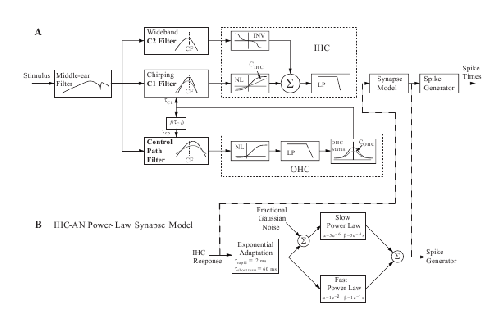
\includegraphics[keepaspectratio=true]{gfx/ZilanyCarney-JASA-2009-Fig2.eps}}
    \caption[Auditory periphery model]{Auditory periphery model with dual power-law synapse
      \citep[originally printed in ][]{ZilanyBruceEtAl:2009}.}
    \label{fig:ZilanyBruceFig}
  \end{center}
\end{figure}\yellownote{if this figure is used it needs permission by the original authors}


\subsection{Spiking in Poisson neural models    \label{sec:CN:spiking-poiss-neur}}

The neural models used in the auditory nerve fibres and Golgi cell model are
inhomogeneous Poisson processes. The instantaneous rate is passed through the
Jackson model, which includes refractory effects typical of the auditory nerve
fibres \citep{Jackson:2003,JacksonCarney:2005}.  Spike trains for each neuron in
the model are created at the start of each repetition of the stimulus, but can
be saved and loaded from file.




% \yellownote{TODO: serious reworking to be done here} 

% Analysis of the frequency
% response area of ANF generates known parameters for each fibre, these are:
% \begin{itemize}
% \item the spontaneous rate (SR), generated in silence and is
%   categoried into two groups High SR ($>$18 sp/s) and Low SR ($<$ 18
%   sp/s);
% \item threshold, the sound pressure level(SPL) at which the cell
%   responds above the spontaneous rate
% \item characteristic frequency (CF)
% \end{itemize}

% \smallskip{}



% \begin{figure}[tbh]
%   \begin{center}
% %     \resizebox{3.5in}{!}{\includegraphics[keepaspectratio=true]{NoFigure}}
% %     \resizebox{3.5in}{!}{\includegraphics[keepaspectratio=true]{ClickDelay}}
%     \caption{Response of AN and CN cells to click stimuli. }
%     \label{fig:ClickDelayAN}
%   \end{center}
% \end{figure}


\section{Cochlear Nucleus Stellate microcircuit    \label{sec:CN:cochl-nucl-stell}}

\subsection{Neural models}


\yellownote{[Discuss R\&M model] Is this a replication of other work or have I changed it enough that it needs to be shown or too general to go in this chapter (put in Methods Chapter}

% \smallskip{}

\subsection{Tonotopic connectivity    \label{sec:CN:tonot-conn}}

The channels are separated using even spatial distance (based on the
basilar membrane and auditory nerve separation) with centre frequency
calculated by the Greenwood function for the cat
\citep{Greenwood:1990}. \yellownote{Expand section on connectivity}

% \smallskip{}

Figure~\ref{fig:CNconn} shows the method for Gaussian spread of
connections between cell types in the \CN\@.  The channels are separated
using the same Greenwood function as used for the AN filterbank.

\begin{figure}[htb]
  \begin{center}
    \resizebox{3.5in}{!}{\includegraphics[keepaspectratio=true]{NoFigure}}
    % \resizebox{\textwidth}{!}{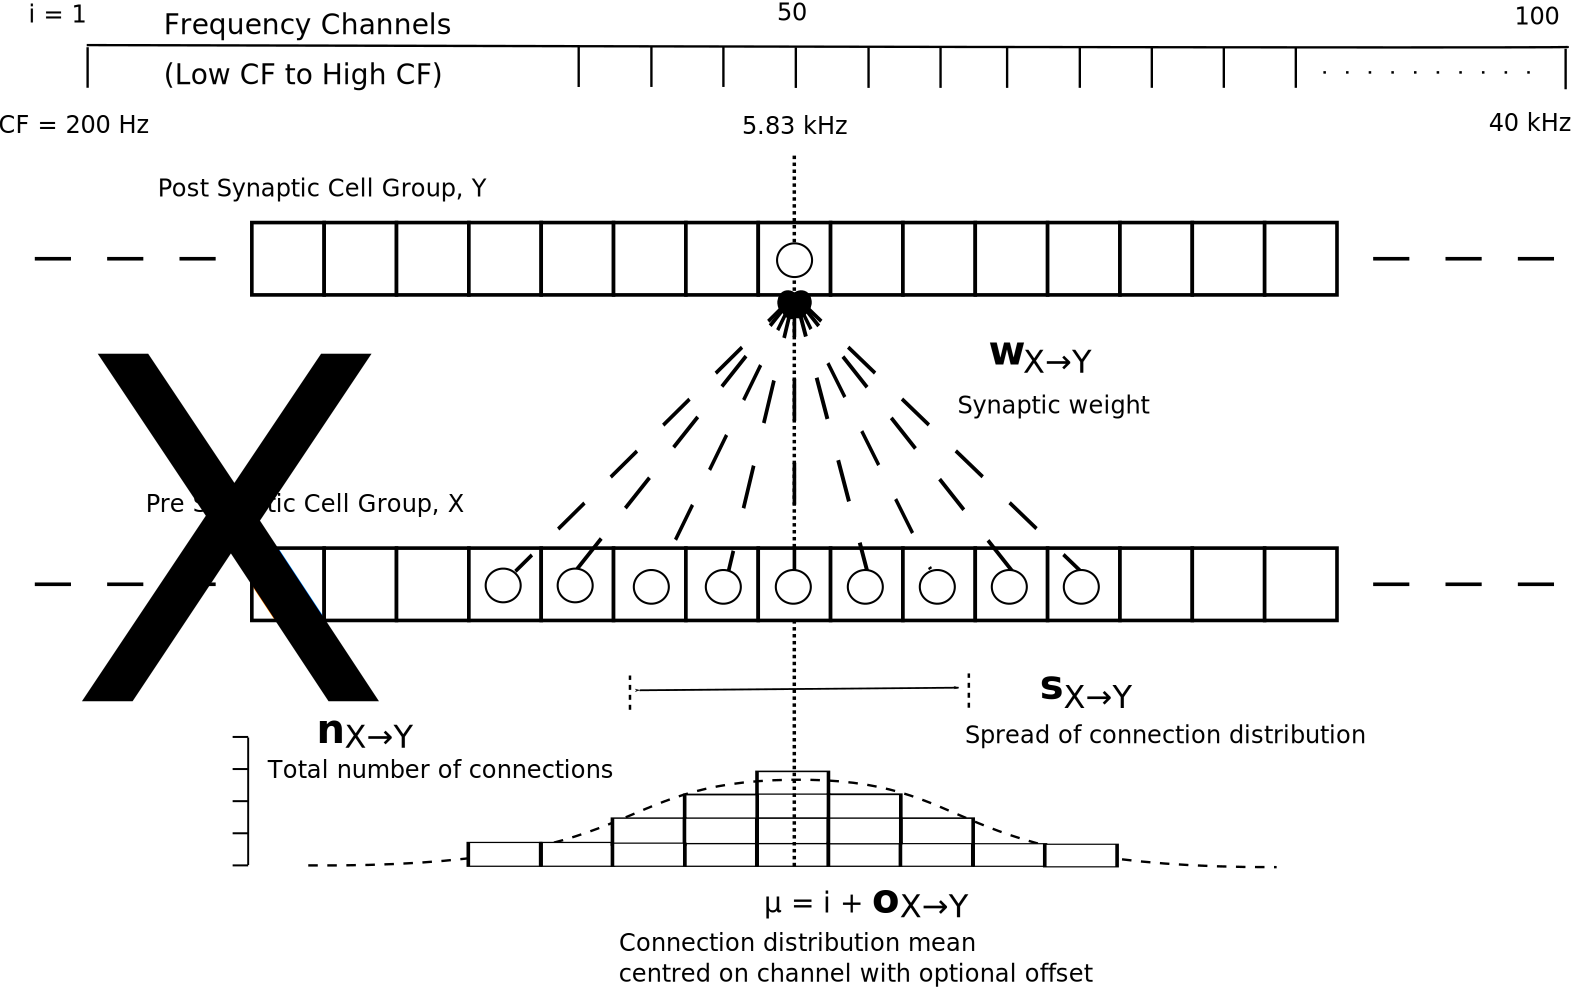
\includegraphics[keepaspectratio=true]{gfx/CNConn}}
    % \resizebox{0.8\textwidth}{!}{\input{./gfx/CNConn.tex}}
    \caption{Diagram    \label{fig:CNdiagram}}
  \end{center}
\end{figure}



\begin{figure}[htb]
  \begin{center}
    % \resizebox{3.5in}{!}{\includegraphics[keepaspectratio=true]{NoFigure}}
    \resizebox{\textwidth}{!}{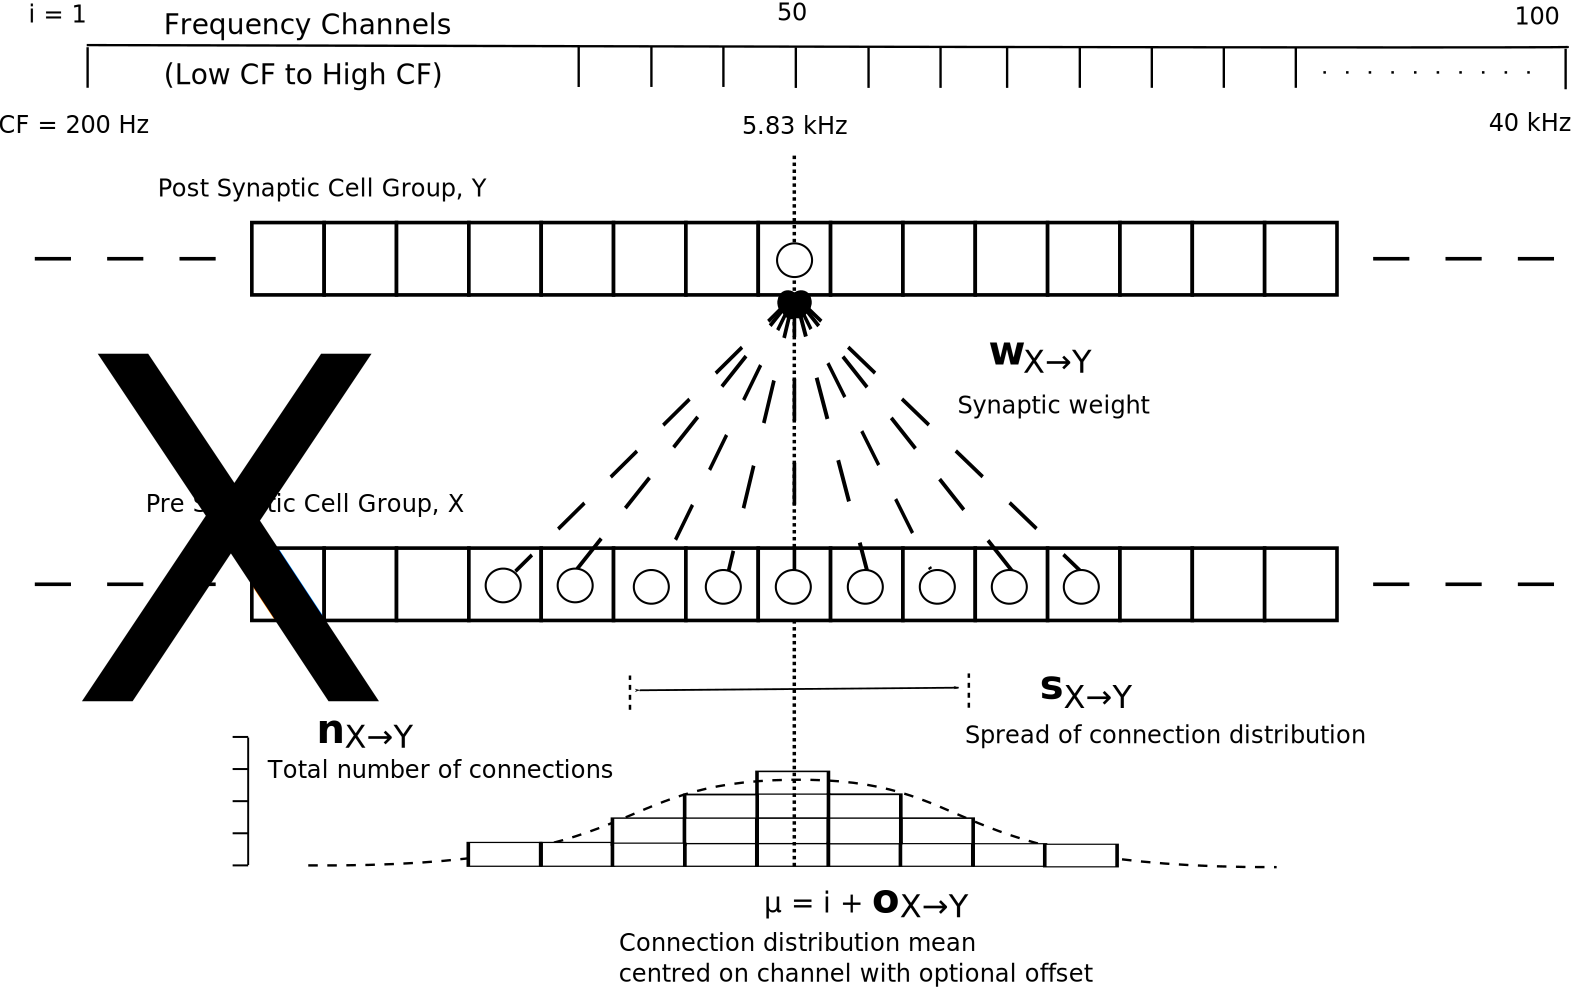
\includegraphics[keepaspectratio=true]{gfx/CNConn}}
    % \resizebox{0.8\textwidth}{!}{\input{./gfx/CNConn.tex}}
    \caption{Gaussian connection between cell types in cochlear
      nucleus.}
    \label{fig:CNconn}
  \end{center}
\end{figure}

% \smallskip{}






%%% Local Variables: 
%%% mode: latex
%%% mode: tex-fold
%%% TeX-master: "SimpleResponses"
%%% TeX-PDF-mode: nil
%%% End: 

\newpage
%===================================
\subsection{Optimisation Results}

Figure~\ref{fig:GolgiTestResult} shows the output of the test optimisation trials for the Golgi cell model.
The testing trial used only five sound levels (0, 15, 55, 75 and 85 dB \SPL) and detected the mean rate from the instantaneous profile in its fitting routine.
The best response obtained a minimum root mean squared error of 11.63 spikes/sec against the five points in the target experimental data of unit S03-07 (CF=21~kHz) from \citep{GhoshalKim:1996}.
A rate-level curve (green circles, Figure~\ref{fig:GolgiTestResult}) was generated from the spiking output only to show a big discrepancy in the spike-based rate-level and the monotonic rate based rate-level.
The lack of low level response and a higher threshold indicated the need for some \HSR~input into the Golgi cell model.

%\smallskip{}


\begin{figure}[htb]
  \centering
\resizebox{0.6\textwidth}{!}{\includegraphics{GolgiRateLevel_result2.eps}}\\
  \caption[Initial results of Golgi cell model]{Initial trial results of the Golgi cell model optimisation.
Responses of the Golgi cell model (blue triangles) compared five five sound level (0,15, 55, 75 and 85 dB SPL) against 5 point in the target response (red squares).
The eventual best optimisation response obtained a minimum error of 11.63 spikes/s (root mean squared).
A spike response (green circles) was generated from the spiking output of the Golgi cell model using the final parameters. \label{fig:GolgiTestResult}}
\end{figure}

The final optimisation routine with 22 levels and a Golgi cell model with \HSR~and \LSR~\ANF~inputs was used to generate a closer fit to the \citeauthor{GhoshalKim:1996}  data.
Figure~\ref{fig:GolgiResult} shows the rate-level output of the best model response and its best combination of parameters are shown in Table~\ref{tab:GolgiCellModelSummary}E.
The root mean squared error of the best response was 4.48~spikes per second.

The parameters in Table~\ref{tab:GolgiCellResults} were within the range of expected values.
\LSR~inputs to the Golgi cell model out-weighted \HSR~inputs by more than a factor of 10.
The monotonic response of \LSR~fibres at high sound levels were necessary to create the large dynamic range in the Golgi cell model, the \HSR~fibres were just as necessary to provide some low level activity.
The spontaneous rate parameter matches the base response of unit S03-07 in Figure~\ref{fig:GolgiResult}.
The smoothing filter time constant of 5 ms is a typical value in membrane time constants for neural models and fits with the input resistance in intracellular recordings of Golgi cells \citep{FerragamoGoldingEtAl:1998}.

The input spread parameter is not well constrained by the optimisation fitness routine with a pure tone input and a single neuron, but the result is satisfactory given the uncertainty in \LSR~fibre's axonal organisation in the \GCD\@. 
The dendritic widths in Golgi cells are around 100 microns and the frequency separation laminae in the \VCN~core is approximately 70 microns, giving an expected result of 1.5 connectivity spread hence the result of 2.48 channels gives added frequency spread from \LSR~fibres.

%\smallskip{}


Table~\ref{tab:GolgiCellModelSummary}E result table.\\
{\small%% Result table
\noindent%
\begin{table}[htb]
  \centering
\begin{tabularx}{\textwidth}{|X|c|c|c|}\hline %{\textwidth}
\hdr{4}{}{GLG model parameters} \\ \hline
                \textbf{Parameters}                 & \textbf{Name} & \textbf{Range} & \textbf{Best Values} \\\hline
     Spatial spread LSR$\to$GLG (channel unit)      &  $\sANFGLG$   &     [0,10]     & 2.48  \\\hline
        Smoothing filter time constant (ms)         &    $\Gtau$    &     [0,20]     & 5.01  \\\hline
          Weighted sum of HSR~(unit-less)           &  $\wHSRGLG$   &     [0,5]      & 0.517 \\\hline
          Weighted sum of LSR~(unit-less)           &  $\wLSRGLG$   &     [0,5]      & 0.0487\\\hline
Spontaneous rate in Golgi cell model (spikes / sec) &   $\Gspon$    &     [0,50]     & 3.73  \\\hline
\end{tabularx}
  \caption{Golgi cell model optimisation parameters}
  \label{tab:GolgiCellResults}
\end{table}
}

\begin{figure}[htb]
  \centering
  % \resizebox{3.5in}{!}{\includegraphics{NoFigure}} \\
\includegraphics[keepaspectratio=true,width=0.6\textwidth]{GolgiRateLevel_result.eps}\\
  % \hspace{1cm}\figfont{A}\hfill\\
  %\resizebox{\textwidth}{!}{\includegraphics{GolgiRateLevel_result2.eps}} \\
  % \hspace{1cm}\figfont{B}\hfill \\
  \caption[Golgi cell model optimisation results]{Golgi cell model optimisation result trials against unit S03-07 (CF 21~kHz) from \citet{GhoshalKim:1996}.
A more detailed optimisation with 22 levels and included HSR inputs in the Golgi cell model generated a closer fit to the Ghoshal and Kim data.
The final root mean squared error was 4.48 spikes/s.
 \label{fig:GolgiResult}}
\end{figure}



%   % \includegraphics[width=0.6\textwidth,angle=-90]{GolgiRateLevelActualFit}\\
%   % \caption{Optimisation Results for Golgi Model using Rate Level data from
%   %     \label{Ch3:fig:GolgiFit}}
%   %   \includegraphics[width=0.8\textwidth]{GolgiRateLevel}\\
%   %   \caption{Optimisation Results for Golgi Model using Rate Level data from
%   %     \label{Ch3:fig:GolgiRL}}

%   %   \includegraphics[width=0.8\textwidth]{golgi_RateLevel_opt}\\
%   %   \caption{Optimisation Results for Golgi Model using Rate Level data from
%   %     \label{Ch3:fig:GolgiRL}}
%   % \includegraphics[width=0.8\textwidth,angle=-90]{GolgiRateLevel2}\\
%     %   \caption{Optimisation Results for Golgi Model using Rate Level data
%     %   from     \label{Ch3:fig:GolgiRL}}
%   \begin{figure}[htb]
%     \centering
% \includegraphics[width=0.6\textwidth,angle=-90]{GolgiRateLevelActualFit}\\
%     \caption{Optimisation Results for Golgi Model using Rate Level data from
%       \label{Ch3:fig:GolgiFit}}
%   \end{figure}
%   \begin{figure}[htb]
%     \centering
%     \includegraphics[width=0.8\textwidth]{GolgiRateLevel}\\
%     \caption{Optimisation Results for Golgi Model using Rate Level data from
%       \label{Ch3:fig:GolgiRL}}
%   \end{figure}
%   \begin{figure}[htb]
%     \centering
%     \includegraphics[width=0.8\textwidth]{golgi_RateLevel_opt}\\
%     \caption{Optimisation Results for Golgi Model using Rate Level data from
%       \label{Ch3:fig:GolgiRL}}
%   \end{figure}
%   \begin{figure}[htb]
%     \centering
% \includegraphics[width=0.8\textwidth,angle=-90]{GolgiRateLevel2}\\
%     \caption{Optimisation Results for Golgi Model using Rate Level data from
%       \label{Ch3:fig:GolgiRL}}
%   \end{figure}

%   \clearpage \newpage

%===================================
\subsection{Verification Results of Golgi Cell Model \label{sec:Golgi:verif-golgi-cell}}
%   \subsubsection{Tone Responses}


After settling with the above optimised parameters, the Golgi cell model was run with typical inputs to determine it's behaviour outside of the optimisation routine.
The Golgi cell model was tested across the entire network using tones, noise and tones plus noise stimuli. Figure~\ref{fig:Golgi_verification}A, B and D show the response of a Golgi cell model at the centre of the network (CF=5.8 kHz) and had monotonic responses to tones and noise similar to other Ghoshal and Kim units (Figure~\ref{fig:GolgiKimFig2}).  Figure~\ref{fig:Golgi_verification}C shows the response of all \GLG units in the network to a 5.8~kHz tone, increased from 0 to 90 dB~{SPL}.
 %\smallskip{}

\begin{figure}[htb]
%\centering
{\figfont{A}\hspace{0.5\textwidth}\figfont{B}\hfill}\\
%\resizebox{0.95\textwidth}{!}{
\includegraphics[keepaspectratio=true,width=0.48\textwidth]{ResponsesNoComp/G_ratelevel_combined.eps}%
\includegraphics[keepaspectratio=true,width=0.48\textwidth]{ResponsesNoComp/RateLevel/psthsingle90.3.eps}\\
%}\\
{\figfont{C}\hspace{0.5\textwidth}\figfont{D}\hfill}\\
%\resizebox{0.95\textwidth}{!}{
\includegraphics[keepaspectratio=true,width=0.48\textwidth]{ResponsesNoComp/RateLevel/response_area.3.eps}%
\includegraphics[keepaspectratio=true,width=0.48\textwidth]{ResponsesNoComp/MaskedResponseCurve3/15/G_masked.eps}\\
%}\\
% }}
%\resizebox{0.45\textwidth}{!}{\includegraphics{ResponsesNoComp/RateLevel/psthsingle90.3.eps}}\\
%\resizebox{0.45\textwidth}{!}{\includegraphics{ResponsesNoComp/RateLevel/psthsingle50.3.eps}}\\
\caption[Optimised Golgi cell model responses]{Response of optimised Golgi cell model at the centre of the network (CF=5.8~kHz). 
A. Rate level responses to tone, noise and tone plus noise. 
B. PSTH at 90 dB~SPL.  
C. Response area equivalent using all GLG units in the network. 
D. Masked noise-tone response of the central unit to 15 dB masking noise and frequencies one octave above and below its CF.} \label{fig:Golgi_verification}
\end{figure}




%   \begin{figure}[h]
%     \centering\resizebox{0.95\textwidth}{!}{%
%     \includegraphics{RateLevel/response_area.3.eps}%
%     \includegraphics{RateLevel/response_area_log2.3.eps}}
%   \end{figure}
%   \begin{figure}[h]
%     \centering\resizebox{0.95\textwidth}{!}{%
%     %     \includegraphics{RateLevel/response_area.3.eps}
%     \includegraphics{RateLevel/psthall90.3.eps}%
%     \includegraphics{RateLevel/psthVlevel.3.eps}}
%   \end{figure}



%   \clearpage
%   \subsubsection{Noise Responses}
%   \begin{figure}[h]
%     \centering\resizebox{0.95\textwidth}{!}{%
%     \includegraphics{NoiseRateLevel/psthsingle120.3.eps}%
%     \includegraphics{NoiseRateLevel/G_ratelevel.eps}}
%   \end{figure}
%   \begin{figure}[h]
%     \centering\resizebox{0.95\textwidth}{!}{%
%     \includegraphics{NoiseRateLevel/response_area.3.eps}%
%     \includegraphics{NoiseRateLevel/response_area_log2.3.eps}}
%   \end{figure}
%   \begin{figure}[h]
%     \centering\resizebox{0.95\textwidth}{!}{%
%     %     \includegraphics{RateLevel/response_area.3.eps}
%     \includegraphics{NoiseRateLevel/psthall90.3.eps}%
%     \includegraphics{NoiseRateLevel/psthVlevel.3.eps}}
%   \end{figure}


%   \clearpage
%   \subsubsection{Masking Responses}
%   \begin{figure}[h!]
% \centering\resizebox{0.95\textwidth}{!}{\includegraphics{MaskedRateLevel/psthsingle90.3.eps}\includegraphics{MaskedRateLevel/G_ratelevel.eps}}
%   \end{figure}
%   \begin{figure}[h!]
%     \centering\resizebox{0.95\textwidth}{!}{%
%     \includegraphics{MaskedRateLevel/response_area.3.eps}%
%     \includegraphics{MaskedRateLevel/response_area_log2.3.eps}}
%   \end{figure}

%   \begin{figure}[h!]
%     \centering\resizebox{0.95\textwidth}{!}{%
%     %     \includegraphics{RateLevel/response_area.3.eps}
%     \includegraphics{MaskedRateLevel/psthall90.3.eps}%
%     \includegraphics{MaskedRateLevel/psthVlevel.3.eps}}
%   \end{figure}
%   \clearpage

%   \begin{figure}[h!]
%     \centering\resizebox{0.95\textwidth}{!}{%
%     \includegraphics{MaskedResponseCurve/psthsingle5810.3.eps}%
%     \includegraphics{MaskedResponseCurve/G_masked.eps}}
%   \end{figure}
%   \begin{figure}[h!]
%     \centering\resizebox{0.95\textwidth}{!}{%
%     \includegraphics{MaskedResponseCurve/response_area.3.eps}%
% \includegraphics{MaskedResponseCurve/response_area_log2log2.3.eps}}
%   \end{figure}

%   \begin{figure}[h!]
%     \centering\resizebox{0.95\textwidth}{!}{%
%     %     \includegraphics{RateLevel/response_area.3.eps}
%     \includegraphics{MaskedResponseCurve/psthall5810.3.eps}%
%     \includegraphics{MaskedResponseCurve/psthVmod.3.eps}}
%   \end{figure}
%   \clearpage


%%% Local Variables:
%%% mode: latex
%%% mode: visual-line
%%% TeX-master: "SimpleResponses"
%%% TeX-PDF-mode: nil
%%% End:

\newpage

\graphicspath{{/media/data/Work/cnstellate/DS_ClickRecovery/}{/media/data/Work/Responses/}}
\section[DS Cell Model]{D-Stellate Cell Model: optimisation using click recovery responses}
\label{sec:d-stellate-cell-model}


This section shows the GABAergic input and intrinsic
cell properties  influence the behaviour Onset chopper units.
Onset-chopper units in the mammalian VCN have a wide-ranging influence
on the primary cells of the VCN (stellate and bushy neurons \citep{RhodeSmithEtAl:1983}), the
ipsilateral DCN (type II and type IV EIRA units) and the contralateral CN \citep{NeedhamPaolini:2007}.  

\medskip{}


% Large multipolar or stellate cells in the VCN have been shown to have
% 3-4 long dendrites stretching 200 microns (or one third of the VCN)
% and their axonal collaterals cover the same region in the VCN, almost
% one half of the DCN, and are one source of the commisural projection
% to the contralateral cochlear nucleus.



%%%%%%%%%%%%%%%%%%%Copied from original jneurometh article



\subsection{Background}

  
D-stelate (DS) cells have an onset-chopping (On-C) PSTH to tones and noise
\citep{SmithRhode:1989,NeedhamPaolini:2006}. Intracellular responses to sounds
indicate the bandwidth of inputs to DS neurons typically ranges from two
octaves below CF to one octave above CF
\citep{PalmerJiangEtAl:1996,PaoliniClark:1999}. DS cell axon terminals contain
the inhibitory neurotransmitter glycine and synapse widely in the VCN and DCN.
They also send a commissural projection to the contralateral cochlear nucleus
that mediates fast inhibition between the nuclei
\citep{NeedhamPaolini:2003,NeedhamPaolini:2006}.  \citep{Oertel:1997}
%%%%%%%%%%%%%%%%%%%%%%%%%%%%%%%%%%%%%%%%%%%%%%%%

Post-onset GABAergic inhibition in DS cells is a major influence on the PSTH
of On-C neurons \citep{FerragamoGoldingEtAl:1998a,EvansZhao:1998}. Latency of
excitation to auditory nerve shocks suggests golgi cells are activated by type
II ANFs and low spontaneous rate type I ANFs
\citep{BensonBerglundEtAl:1996,FerragamoGoldingEtAl:1998}. Therefore, type II
and LS type I ANFs could be involved in gain control through GABAergic
modulation of activity in the VCN.


\medskip{}

[Discuss AM coding by DS cells]
\citep{CasparyPalombiEtAl:2002} GABA blockers in the VCN has the effects of changing the behaviour in the response to AM in the IC.
\citep{BackoffShadduckEtAl:1999} AM coding effects of GABA in the Chinchilla CN.
\citep{CasparyBackoffEtAl:1994}
Caspary et al. worked on the effects of GABA in in the VCN. 

Zhang and Winter looked at the response area of VCN onset units to determine GABA on/off freq

Smith and Rhode, Smith et al. looked at OnC respnse area and two-tone



\subsection{Implementation}
 
Key factors in designing D-stellate cell model

\medskip{}

Choosing neural model: type I-II Rothman and Manis model
  - with/without dendrites
  - variable KLT, leak conductance

\begin{itemize}
\item  ANF spread to DS cells well documented (decision made to
    fix params due to large computational task of calc response area) 
\item  short delay recovery responses (2,3,4 ms) were not successful upon
    first model, included DS leak and KLT conductances to allow cell
    behaviour to be fit
  \item The effect of Golgi cells on DS is delayed by the extra 0.7 ms
    delay from ANF to Golgi, plus the slow peak of \GABAa inhibition.
\end{itemize}

\medskip{}

Optimisation parameters for \GLGDS are optimised based on experimental
click recovery data from \citep{BackoffPalombiEtAl:1997}.  Fixed
parameters included the number of golgi cells to DS cells ($\nGLGDS =
25$), the spread of ANFs to DS cells $\ANFDS$, and the extra delay from the auditory
nerve.  The first spike latency in DS cells 2.8 ± 0.09 ms
\citep{RhodeSmith:1986}.The addition of 0.5 ms to \ANFDS connections
is a combination of conductance and synaptic delay. The effect of
Golgi cells on DS is delayed by the extra 0.7~ms delay from ANF to
Golgi, plus the slow peak of \GABAa inhibition.  
The spread ANF to DS cells (\sANFDSh,\sANFDSl) is arbitrary at this point and fairly broad so the
estimate is set so that 2 octaves below and 1 octave above CF are
within 2 standard deviations \citep{PaoliniClark:1999}.

\medskip{}

The optimisation function was a weighted mean squared error between
the experimental and simulated data, from an array where the elements
were the number of spikes in a 2 ms window after a click.  The input
stimulus was a series of masker/response clicks, with the click
intervals of 2, 3, 4, 8, 16 ms, and a separation of 50 ms.


\noindent
\begin{tabularx}{\textwidth}{|l|X|}\hline %
%
\hdr{2}{A}{Model Summary}\\\hline
\textbf{Populations}     & ANF (HSR,LSR), Golgi, D-stellate \\\hline
\textbf{Topology}        & Tonotopic,  Auditory system of the rat  \\\hline
\textbf{Connectivity}    & Gaussian spread dependent on morphology and afferent connections  \\\hline
\textbf{Input model}  &  ANF phenomenological instantaneous-rate Poisson spike trains\citep{ZilanyBruceEtAl:2009}\\\hline
\multirow{2}{*}{\textbf{Neuron model}}    & Golgi: instantaneous-rate Poisson spike trains\\
&D-stellate: HH-like single-compartment model (Type 1-2 RM model)\\ \hline
\textbf{Channel models}  & $I_{\textrm{Na}}$, $I_{\textrm{KHT}}$, $I_{\textrm{KLT}}$, $I_{\textrm{KA}}$ and $I_{\textrm{h}}$ \citep{RothmanManis:2003b} \\\hline
\textbf{Synapse model}   & Conductance synapses: excitatory (single-exponential), GABAergic (double-exponential) \\\hline
\textbf{Input Stimulus}  & Mask/Recovery click trains with delay 2, 3, 4 and 8
ms, separated by 50 ms\\\hline
\textbf{Measurements}    & PSTH sampled at each recovery click for 2 ms to measure click recovery\\\hline
\end{tabularx}
\vspace{2ex}

% - B -----------------------------------------------------------------------------

\noindent
\begin{tabularx}{\textwidth}{|l|X|X|}\hline %{\textwidth}
\hdr{3}{B}{Populations}\\\hline
\textbf{Name} &            \textbf{Elements}            & \textbf{Number} \\\hline
     HSR      &            Poisson generator with refractory effects           & $N_{\text{HSR}} = 50$ per freq.\ channel \\\hline
     LSR      &            ''            & $N_{\text{LSR}}= 20$  per freq.\ channel \\\hline
     GLG      &            ''            & $N_{\text{GLG}}= 1$  per freq.\ channel  \\\hline
     DS       &  Type I-II RM model & $N_{\text{DS}}= 1$ at CF=5.6~kHz \\\hline
\end{tabularx}
\vspace{2ex}

% - C ------------------------------------------------------------------------------

\noindent
\begin{tabularx}{\textwidth}{|l|l|l|X|}\hline
\hdr{4}{C}{Connectivity}\\\hline
        \textbf{Name}          &  \textbf{Source}  & \textbf{Target} & \textbf{Pattern} \\\hline
$\textrm{ANF} \to \textrm{DS}$ & ANF (HSR and LSR) &   D-Stellate    & skewed Gaussian, centered at CF, spread below CF \sANFDSl, spread above CF \sANFDSh, uniform weight \wANFDS for all synapses, number \nLSRDS and \nHSRDS, delay \dANFDS \\\hline
$\textrm{GLG} \to \textrm{DS}$ &       Golgi       &   D-Stellate    & Gaussian, centered at CF with spread \sGLGDS, uniform weight \wGLGDS, number \nGLGDS, delay \dGLGDS \\\hline
\end{tabularx}

\vspace{2ex}




% - D ------------------------------------------------------------------------------



%\noindent\begin{tabularx}{\textwidth}{|p{0.150.95\textwidth}|X|}\hline
%\hdr{2}{D}{Neuron and Synapse Model}\\\hline
% \textbf{Name} & Poisson spike generator \\\hline
% \textbf{Type} & Leaky integrate-and-fire, $\delta$-current input\\\hline
% \raisebox{-4.5ex}{\parbox{\textwidth}{\textbf{Subthreshold dynamics}}} &
% \rule{1em}{0em}\vspace*{-3.5ex}
%     \begin{equation*}
%       \begin{array}{r@{\;=\;}lll}
% \tau \dot{V}(t) & -V(t) + R I(t) & \text{if} & t > t^*+\tau_{\text{rp}} \\
%      V(t)       &  V_{\text{r}}  & \text{else} \\[2ex]
%      I(t)       & \multicolumn{3}{l}{\frac{\tau}{R} \sum_{\tilde{t}} w \delta(t-(\tilde{t}+\Delta))}
% \end{array}
%     \end{equation*}
% \vspace*{-2.5ex}\rule{1em}{0em}
%  \\\hline
 % \multirow{3}{*}{\textbf{Spiking}} &   If $V(t-)<\theta \wedge V(t+)\geq \theta$ \vspace*{-1ex}
 % \begin{enumerate}\setlength{\itemsep}{-0.5ex}
 % \item set $t^* = t$
 % \item emit spike with time-stamp $t^*$
 % \end{enumerate}
 % \vspace*{-4ex}\rule{1em}{0em} \\\hline
 % \end{tabularx}

\vspace{2ex}

% - E ------------------------------------------------------------------------------

\noindent
\begin{tabularx}{\textwidth}{|X|c|c|c|}\hline %{\textwidth}
\hdr{4}{E}{Optimisation} \\ \hline
     \textbf{Parameters}      &  \textbf{Name}   &        \textbf{Range}         & \textbf{Best Values} \\\hline 
     Weight of GLG on DS (nS)      &     \wGLGDS      &         [0.01,50]          & 0.532 \\	\hline	
   Weight of HSR syn on DS (nS)	  &	\wHSRDS	     &		[0.01,50]	   & 0.16 \\	   \hline
   Weight of LSR syn on DS  (nS)  &	\wLSRDS	     &		[0.01,50]	   & 13.1 \\	    \hline
\GABAa synapse rise constant  (ms)&  $\tau_{GABA1}$  &	       [0.01,10.0]	   & 5.432\\	     \hline
\GABAa synapse decay constant (ms)&  $\tau_{GABA2}$  &	       [0.1,50.0]	   & 0.262\\	    \hline
  DS cell leak conductance (mS per cm$^2$)   & $\bar{g}_{leak}$ & [1e-5,5e-2]  & 0.0163 \\ \hline
\end{tabularx}
\vspace{2ex}




% - F -----------------------------------------------------------------------------

\noindent\begin{tabularx}{\textwidth}{|X|}\hline
  \hdr{1}{F}{Measurements}\\\hline 
PSTHs were generated from 25
  stimulus repetitions. Each response to a click is measured for 2 ms
  after the minimum first spike latency for the unit.  The unit used
  in the optimisation has a CF = 5.8~kHz (channel no. 50).\\ \hline
% \begin{minipage}[c]{0.6\textwidth}
% \vspace{1cm}
% DS Ouput \hspace{2in} Golgi Output
% %\includegraphics[width=0.5\textwidth]{DS_ClickRecovery_DSpsth}\label{Ch3:fig:DSClickRecoveryPSTH}\includegraphics[width=0.5\textwidth]{DS_ClickRecovery_Gpsth}\label{Ch3:fig:DSClickRecoveryPSTH}\\
%   \captionsize{PSTH response of a D-stellate cell from the click recovery stimulus used in the optimisation.}
%   \end{minipage}\\ \hline
\end{tabularx}

 % ---------------------------------------------------------------------------------
% \newpage
% \begin{lstlisting}
% func fun() {local f
%       //Modify Variables
%       param.w.x[glg][ds] = $2
%       param.w.x[hsr][ds] = $3
%       param.w.x[lsr][ds] = $3
%       //Modify the network
%       {create_cells() connect_cells(fileroot) SetRates()}
%       // Simulate the network for N reps
%       for j=0, reps-1{
%          print j
%          GenSpikes()
%          run()
%          DSvec.append(dstellate[50][0].spiketimes)
%          //print startsw()-x, "secs"
%       }
%       DSvec = DSvec.histogram(0,tstop,0.1)
%
%       objref errorvec
%       errorvec = new Vector()
%       //Find the mean number of spikes in the first click
%       maxrate = (DSvec.sum(240,260) + DSvec.sum(740,760)+ DSvec.sum(1340,1360))/3
%       //Calc ratio of number of spikes in second click relative to mean first click
%       errorvec.append( DSvec.sum(260,280) / maxrate )
%       errorvec.append( DSvec.sum(780,800) / maxrate )
%       errorvec.append( DSvec.sum(1420,1440) / maxrate )
%       errorvec.plot(g
%     return errorvec.meansqerr(targetclick)
% }
% \end{lstlisting}











\begin{figure}[htb]
\includegraphics[angle=-90,width=0.8\textwidth]{DSClickRecoveryExpData}\label{Ch3:fig:DSClickRecoveryExpData}
\caption{Experimental Data of GABAergic influence on D-stellate cells from \citep{BackoffPalombiEtAl:1997}, Fig.~3.}
\end{figure}

%\parsep

% From the command line type:
% \begin{verbatim}
% $ ./i686/special DS_ClickRecovery.hoc
% \end{verbatim}
% in the \texttt{cnstellate} directory to simulate the optimisation for D-stellate click recovery.  The first run may take some time if the AN filters have not been previously saved, since the Zilany \& Bruce model requires 500~kHz resolution in the stimulus that is downsampled to 50~kHz.

\clearpage
\subsection{Results}


% \noindent\begin{tabularx}{\textwidth}{|l|X|}\hline %{\textwidth}
% \hdr{2}{D}{Results} \\\hline
% \end{minipage}}\\\hline
% \textbf{Error} & 0.006671    unweighted (MSE of recovery spike rate / mask rate)\\\hline
% & 0.01447    final result (MSE of recovery spike rate / mask rate)\\\hline
% \end{tabularx}

\begin{figure}[hp!]
  \centering
\includegraphics[keepaspectratio=true,angle=-90,width=0.9\textwidth]{./gfx/DS_ClickRecovery_result.eps}
%\includegraphics[keepaspectratio,angle=-90,width=0.8\textwidth]{./gfx/DSClickRecoveryExpData}\\
\caption{Experimental Data ({\color{green} Green}) of GABAergic influence on D-stellate cells from \citep{BackoffPalombiEtAl:1997}, Fig.~3.  Best result ({\color{blue} Blue}) shown in figure below. }
\label{fig:DS_ClickRecovery_result}  
\end{figure}


% \begin{figure}
%   \includegraphics[width=0.5\textwidth]{DS_ClickRecovery_OptVars.eps}\\
% %  \includegraphics[width=0.5\textwidth]{DS_ClickRecovery_Output.eps}\label{Ch3:fig:DSClickRecoveryOutput}
%   \caption{Final Output Data of the D-stellate Click Recovery optimisation }
% \end{figure}

% \begin{figure}
%   \includegraphics[keepaspectratio=true,width=0.8\textwidth]{DS_ClickRecovery_Example1.eps}\\
%   \includegraphics[keepaspectratio=true,width=0.8\textwidth]{DS_ClickRecovery_Example10.eps}\\
%   \includegraphics[keepaspectratio=true,width=0.8\textwidth]{DS_ClickRecovery_Example13.eps}\\
%   \includegraphics[keepaspectratio=true,width=0.8\textwidth]{DS_ClickRecovery_Example19.eps}\\
%   \caption{Click Recovery optimisation functions}
% \end{figure}


% \begin{figure}
%   \includegraphics[keepaspectratio=true,angle=-90,width=0.8\textwidth]{DS_ClickRecovery_result.eps}\\
% \end{figure}


% \begin{figure}
%   \includegraphics[keepaspectratio=true,angle=-90,width=0.8\textwidth]{DS_ClickRecovery_result1.eps}\\
% \end{figure}


% \begin{figure}
%   \includegraphics[keepaspectratio=true,angle=-90,width=0.8\textwidth]{DS_ClickRecovery_result2.eps}\\
%   \caption{Click Recovery optimisation }
% \end{figure}




% \begin{figure}
% \begin{center}
% \includegraphics[keepaspectratio=true]{DS_ClickRecovery_handtuned.eps}\\
% \includegraphics[keepaspectratio=true,angle=-90,width=0.8\textwidth]{DS_ClickRecovery_result_handtuned.eps}
% \caption{Handtuned}
% \label{hantuned}
% \end{center}
% \end{figure}

% \begin{figure}
% \begin{center}
% %\includegraphics[keepaspectratio=true]{DS_ClickRecovery_handtuned.eps}\\
% \includegraphics[keepaspectratio=true,angle=-90,width=0.8\textwidth]{gfx/DS_ClickRecovery_result_unweighted_8.eps}\\
% \includegraphics[keepaspectratio=true,angle=-90,width=0.8\textwidth]{gfx/DS_ClickRecovery_result_weighted_0.eps}
% \caption{Handtuned}
% \label{hantuned}
% \end{center}
% \end{figure}


%% Example optimisation points used by praxis 
% \begin{figure}
% \begin{center}
% %\includegraphics[keepaspectratio=true]{DS_ClickRecovery_handtuned.eps}\\
% \includegraphics[keepaspectratio=true,width=0.5\textwidth]{Praxis_123.eps}
% \includegraphics[keepaspectratio=true,width=0.5\textwidth]{Praxis_456.eps}
% \caption{Handtuned}
% \label{hantuned}
% \end{center}
% \end{figure}


% \clearpage
\newpage
\subsection{Verification}

 \subsection{Tone Response}
% \begin{figure}[h!]
% \centering\resizebox{\textwidth}{!}{%
% \includegraphics{RateLevel/psthsingle90.2.eps}%
% \includegraphics{RateLevel/DS_ratelevel.eps}}
% \end{figure}
% \begin{figure}[h!]
% \centering\resizebox{\textwidth}{!}{%
% \includegraphics{RateLevel/response_area.2.eps}%
% \includegraphics{RateLevel/response_area_log2.2.eps}}
% \end{figure}
% \begin{figure}[h!]
% \centering\resizebox{\textwidth}{!}{%
% %\includegraphics{RateLevel/response_area.2.eps}
% \includegraphics{RateLevel/psthall90.2.eps}%
% \includegraphics{RateLevel/psthVlevel.2.eps}}
% \end{figure}


% \clearpage
 \subsection{Noise Response}
% \begin{figure}[h!]
% \centering\resizebox{\textwidth}{!}{%
% \includegraphics{NoiseRateLevel/psthsingle120.2.eps}%
% \includegraphics{NoiseRateLevel/DS_ratelevel.eps}}
% \end{figure}
% \begin{figure}[h!]
% \centering\resizebox{\textwidth}{!}{%
% \includegraphics{NoiseRateLevel/response_area.2.eps}%
% \includegraphics{NoiseRateLevel/response_area_log2.2.eps}}
% \end{figure}
% \begin{figure}[h!]
% \centering\resizebox{\textwidth}{!}{%
% %\includegraphics{RateLevel/response_area.2.eps}
% \includegraphics{NoiseRateLevel/psthall90.2.eps}%
% \includegraphics{NoiseRateLevel/psthVlevel.2.eps}}
% \end{figure}


% \clearpage
 \subsection{Masked Noise and Tone}
% \begin{figure}[h!]
% \centering\resizebox{\textwidth}{!}{\includegraphics{MaskedRateLevel/psthsingle90.2.eps}\includegraphics{MaskedRateLevel/DS_ratelevel.eps}}
% \end{figure}
% \begin{figure}[h!]
% \centering\resizebox{\textwidth}{!}{%
% \includegraphics{MaskedRateLevel/response_area.2.eps}%
% \includegraphics{MaskedRateLevel/response_area_log2.2.eps}}
% \end{figure}

% \begin{figure}[h!]
% \centering\resizebox{\textwidth}{!}{%
% %\includegraphics{RateLevel/response_area.2.eps}
% \includegraphics{MaskedRateLevel/psthall90.2.eps}%
% \includegraphics{MaskedRateLevel/psthVlevel.2.eps}}
% \end{figure}
% \clearpage
 \subsection{Masked Response Area}
% \begin{figure}[h!]
% \centering\resizebox{\textwidth}{!}{%
% \includegraphics{MaskedResponseCurve/psthsingle5810.2.eps}%
% \includegraphics{MaskedResponseCurve/DS_masked.eps}}
% \end{figure}
% \begin{figure}[h!]
% \centering\resizebox{\textwidth}{!}{%
% \includegraphics{MaskedResponseCurve/response_area.2.eps}%
% \includegraphics{MaskedResponseCurve/response_area_log2log2.2.eps}}
% \end{figure}

% \begin{figure}[h!] 
% \centering\resizebox{\textwidth}{!}{%
% %\includegraphics{RateLevel/response_area.2.eps}
% \includegraphics{MaskedResponseCurve/psthall5810.2.eps}%
% \includegraphics{MaskedResponseCurve/psthVmod.2.eps}}
% \end{figure}
% \clearpage

 

%%% Local Variables: 
%%% mode: latex
%%% TeX-master: "SimpleResponses"
%%% TeX-PDF-mode: nil
%%% End: 

\newpage

\graphicspath{{/media/data/Work/cnstellate/TV_notch/}{/media/data/Work/Responses/}{/media/data/Work/cnstellate/}{/media/data/Work/thesis/ans2010/gfx/}}
\newpage
\section[TV Cell Model]{Tuberculo-ventral cell model: Asymmetric broadband inhibition }
\label{sec:tv-cell-model}
% - A ------------------------------------------------------------------------------

\subsection{Background}

Tuberculoventral (TV) cells are glycinergic, inhibitory cells found in
the deep layers of the DCN that send axon collaterals to the VCN\@. They
are characterized as having a non-monotonic response to tones with
increasing sound level and respond poorly to broadband noise
\citep{SpirouDavisEtAl:1999,NelkenYoung:1997,ReissYoung:2005}.
Anterograde labeling in the DCN suggests TV cells project
tonotopically to the AVCN not just on-CF, but also to the low and high
frequency side bands in the AVCN
\citep{MunirathinamOstapoffEtAl:2004,OstapoffMorestEtAl:1999}.
Ultra-structural labeling of synapses in the rat DCN suggest TV cells
are inhibited by glycinergic DS cells and from sources in the DCN but
excitatory inputs were not found from TS cells in the rat
\citep{Rubio:2005}. Evidence in the mouse suggests otherwise since
intracellular responses from labeled TV cells in the mouse show clear
excitatory input from TS cells and diffuse inhibitory input from DS
cells \citep{ZhangOertel:1993b,WickesbergOertel:1993}.



\quote{ \emph{Spirou}

Vertical cells receive monosynaptic excitatory input from au-
ditory nerve fibers (Oertel and Wu 1989; Zhang and Oertel
1993b). Taken together, these two results suggest that low SR
auditory nerve fibers may form the major excitatory input to
type II cells. If true, this hypothesis also could explain the
finding that type II units have consistently higher thresholds
than DCN principal cells (Young and Brownell 1976) because
low SR auditory nerve fibers also have elevated thresholds
relative to the lowest threshold auditory nerve fibers (Liberman
1978). However, patterns of auditory nerve innervation of the
DCN are most consistent with high SR fiber innervation of
vertical cell somata and low SR fiber innervation of dendrites
(Liberman 1993). In that case, the low spontaneous rates and
high sound thresholds of type II units might be caused by a
high intrinsic electrical threshold (Hancock et al. 1997); this is
consistent with the responses of vertical cells to intracellular
current injection (Ding and Voigt 1997; Zhang and Oertel
1993b).


...
Type II units also supply an inhibitory input to the VCN
(Wickesberg and Oertel 1990), but the role of type II terminals
in the VCN is less clear. Three different hypotheses have been
raised. The first is that this projection modulates the response
thresholds of VCN neurons (Paolini et al. 1998). This hypoth-
The role of type II units in spectral processing is that of a
narrowband inhibitor. Responses of DCN principal cells are
strongly inhibited by this narrowband source. As a result, DCN
principal cells are inhibited by sharp spectral peaks close to
their BF.

type II units. Thus if onset-C units are not the inhibitory input
to type II units, then the actual inhibitor should have properties
identical to the onset-C unit.

Synaptic organization: unresolved issues

Despite the coherent picture developed in the preceding text,
there are some remaining uncertainties about type II synaptic
organization. First, there are few inhibitory puncta on the
somata of vertical cells, in comparison with DCN principal
cells, (Osen 1990; Saint Marie et al. 1991) and little sign of
disynaptic IPSPs in vertical cells after auditory-nerve stimula-
tion in slice preparations (Zhang and Oertel 1993b). Thus
current anatomic and in vitro studies do not provide a basis for
the strong inhibition seen physiologically. Second, the radiate
(D-stellate) neurons are glycinergic (Doucet et al. 1999), but the
noise-driven inhibition of type II units is reduced significantly
by bicuculline as well as by strychnine (Fig. 8). The sensitivity
of DCN cells to GABA antagonists has been reported before
(Caspary et al. 1987; Evans and Zhou 1993). It seems likely
that there are GABAergic inhibitory inputs on type II units, in
addition to the glycinergic inputs from radiate neurons. The
source of these GABAergic inputs is not known, although there
are many GABAergic cells in the cochlear nucleus (Kolston et
al. 1992; Osen et al. 1990) as well as GABAergic projections
from the superior olivary complex (Ostapoff et al. 1990, 1997).
Third, the evidence from two-tone response maps, inhibitory
blockade, and noiseband widening suggests that the inhibition
in type II units is centered on or near BF; models of type II
responses assume the same thing. However, it is not clear that
D-stellate cells project in a tonotopic fashion; indeed, injections
of tracer into circumscribed regions of the tonotopic map of
DCN fill radiate cells across a wide range of the tonotopic map
in VCN (Doucet and Ryugo 1997). Thus it is not clear how the
apparent tonotopic projection of the wideband inhibitor would
correspond to the apparently nontonotopic projection of radiate
neurons. Because the details of the anatomic circuitry of the
deep DCN are largely unknown, the relevance of these points
cannot be properly evaluated at present. More information
about the anatomic inputs to vertical cells, especially their
dendritic inputs, is required.

Functional role of type II units
The role of type II units in spectral processing is that of a
narrowband inhibitor. Responses of DCN principal cells are
strongly inhibited by this narrowband source. As a result, DCN
principal cells are inhibited by sharp spectral peaks close to
their BF. These units also are inhibited by a wideband source,
probably the onset-C neuron (Nelken and Young 1994), which
produces the inhibition seen in principal cells in response to
notches in the stimulus spectrum (Spirou and Young 1991;
Young et al. 1992). Thus type II cells participate in the con-
struction of the exquisite sensitivity of DCN principal cells to
sharp spectral features, both peaks and notches.
Type II units also supply an inhibitory input to the VCN
(Wickesberg and Oertel 1990), but the role of type II terminals
in the VCN is less clear. Three different hypotheses have been
raised. The first is that this projection modulates the response
thresholds of VCN neurons (Paolini et al. 1998). This hypoth-
esis is based on the finding that vertical cells provide a tono-
topically organized inhibitory input to bushy and stellate neu-
rons of the VCN (Wickesberg and Oertel 1990) and on the
finding that injection of the GABA agonist muscimol into DCN
produced a significant lowering of the average threshold of
VCN units (Paolini et al. 1998). The advantage of having VCN
thresholds elevated in this way by DCN activity is not clear;
moreover, the properties of the threshold elevation do not
correspond to those of type II units, which are not spontane-
ously active and have high-thresholds themselves. Thus the
role of type II units in modulating VCN thresholds is not clear.
The second hypothesis is that the inhibitory projection from
DCN to VCN produces monaural echo suppression (Wickes-
berg and Oertel 1990). This hypothesis is based on the finding
that vertical cells supply a delayed, frequency specific input to
the VCN. Two-click data (Wickesberg 1996) provide partial
physiological support for this idea, but only 19% of VCN cells
showed the expected increase in response to the second click
after lidocaine injections in DCN. In general, the role of type
II units in temporal processing is hard to interpret because their
temporal properties are complex and nonlinear (Joris and
Smith 1998).

The third hypothesis on the role of the type II projection to
VCN is that it helps to reduce the effects of spectral notches
caused by the acoustical properties of the pinnae (Rice et al.
1992) on the representation of complex sounds in the VCN
(Nelken and Young 1996). Unlike DCN neurons, VCN cells
are not inhibited by narrow spectral peaks or notches. Presum-
ably the inhibition from type II units is too weak in VCN to
produce the effects that are seen in DCN. Instead the tonotopic
array of type II neurons weakly inhibits VCN principal cells
except in the region of the notch itself. The result is an
enhancement of the spectral information in the notch relative to
its surround, essentially counteracting the effects of pinna
acoustics in producing the spectral notch. In this way, infor-
mation about the notch itself would be conveyed in the outputs
of the DCN and information about the spectral shape of the
stimulus would be conveyed by the outputs of the VCN.
Type II neurons may participate in all the functions proposed
in the preceding text, but more information about their con-
nections and responses to complex stimuli are required to fully
evaluate these hypotheses. Nevertheless, the accumulated
physiological and anatomic evidence indicate that type II neu-
rons play an important role in establishing the response prop-
erties of a wide variety of cochlear nucleus neurons, and thus
they play a crucial role in the transformations of the auditory
representation that take place in the cochlear nucleus.





}


\subsection{Implementation}

\noindent\begin{tabularx}{\textwidth}{|l|X|}\hline %
\hdr{2}{A}{Model Summary}\\\hline
\textbf{Populations}     & Five: HSR \& LSR ANFs, Golgi, DS, and TV cells \\\hline
\textbf{Topology}        & Tono-topicity of the rat AN and CN \\\hline
\textbf{Connectivity}    & ANF$\to${Golgi,DS,TV}, Golgi$\to$DS, DS$\to$TV  \\\hline
\textbf{Neuron model}    &\begin{minipage}{0.5\textwidth}
Golgi cell \begin{itemize}
\item instantaneous-rate Poisson spike trains
\item weighted sum of LSR instantaneous-rate vectors
\item smoothing due to alpha function kernel
\end{itemize}
D-stellate cell\begin{itemize}
\item biophysically-based HH-like single-compartment model
\item type I-II current-clamp model
\end{itemize}
Tuberculo-ventral cell \begin{itemize}
\item biophysically-based HH-like single-compartment model
\item type I-c current-clamp model \citep{RothmanManis:2003b}
\end{itemize}
\end{minipage}\\\hline
\textbf{Channel models}  &  $I_{\textrm{Na}}$, $I_{\textrm{KHT}}$, $I_{\textrm{KLT}}$, $I_{\textrm{KA}}$ and $I_{\textrm{h}}$ \citep{RothmanManis:2003b}\\\hline
\textbf{Synapse model}   & AMPA (\textit{ExpSyn}), GABA$_{\rm A}$ (\textit{Exp2Syn}), Glycine (\textit{Exp2Syn}) \\\hline
\textbf{Input}           &  Notch-noise (Stop-band filtered white noise) \\\hline
\textbf{Measurements}    &  First spikes and PSTH of TV cells, calculated for first spike latency, mean rate and variance \\\hline
\end{tabularx}

\vspace{2ex}

% - B -----------------------------------------------------------------------------

\noindent\begin{tabularx}{\textwidth}{|l|l|X|}\hline
\hdr{3}{B}{Populations}\\\hline
\textbf{Name} &    \textbf{Elements}    & \textbf{Size} \\\hline
     HSR      &    Poisson generator    & $N_{\text{HSR}} = 50$ per freq.\ channel \\\hline
     LSR      &    Poisson generator    & $N_{\text{LSR}}= 20$  per freq.\ channel \\\hline
     GLG      &    Poisson generator    & $N_{\text{GLG}}= 1$  per freq.\ channel  \\\hline
     DS       &   Type I-II RM model    & $N_{\text{DS}}= 1$ per freq\. channel \\\hline
     TV       & Type I-classic RM model & $N_{\text{TV}}= 1$ per freq\. channel\\\hline
\end{tabularx}

\vspace{2ex}

% - C ------------------------------------------------------------------------------

\noindent\begin{tabularx}{\textwidth}{|l|l|l|X|}\hline
\hdr{4}{C}{Connectivity}\\\hline
\textbf{Name} &  \textbf{Source}  & \textbf{Target}  & \textbf{Pattern} \\\hline
   \ANFDS     & ANF (HSR and LSR) &    D-Stellate    & skewed Gaussian, centered at CF, spread below CF \sANFDSl, spread above CF \sANFDSh, uniform weight \wANFDS for all synapses, number \nLSRDS \& \nHSRDS, delay \dANFDS \\\hline
   \ANFTV     & ANF (HSR and LSR) & Tuberculoventral & Narrowband, centered at CF,spread negligent , uniform weight \wANFDS for all synapses, number \nLSRDS \& \nHSRDS, delay \dANFDS \\\hline
   \GLGDS     &       Golgi       &    D-Stellate    & Gaussian, centered at CF with spread \sGLGDS, uniform weight \wGLGDS, number \nGLGDS, delay \dGLGDS \\\hline
    \DSTV     &    D-Stellate     & Tuberculoventral & Gaussian, centered at CF with spread \sGLGDS, uniform weight \wGLGDS, number \nGLGDS, delay \dGLGDS \\\hline
\end{tabularx}

\vspace{2ex}

% - D ------------------------------------------------------------------------------

% \noindent\begin{tabularx}{\textwidth}{|p{0.150.95\textwidth}|X|}\hline
% \hdr{2}{D}{Neuron and Synapse Model}\\\hline
% \textbf{Name} &  \\\hline
% \textbf{Type} & \\\hline
% \raisebox{-4.5ex}{\parbox{0.95\textwidth}{\textbf{Subthreshold dynamics}}} &
% \rule{1em}{0em}\vspace*{-3.5ex}
%     \begin{equation*}
%       \begin{array}{r@{\;=\;}lll}
%       \tau \dot{V}(t) & -V(t) + R I(t) &\text{if} & t > t^*+\tau_{\text{rp}} \\
%       V(t) & V_{\text{r}} & \text{else} \\[2ex]
%       I(t) & \multicolumn{3}{l}{\frac{\tau}{R} \sum_{\tilde{t}} w
%         \delta(t-(\tilde{t}+\Delta))}
%       \end{array}
%     \end{equation*}
% \vspace*{-2.5ex}\rule{1em}{0em}
%  \\\hline
% \multirow{3}{*}{\textbf{Spiking}} &
%    If $V(t-)<\theta \wedge V(t+)\geq \theta$
% \vspace*{-1ex}
% \begin{enumerate}\setlength{\itemsep}{-0.5ex}
% \item set $t^* = t$
% \item emit spike with time-stamp $t^*$
% \end{enumerate}
% \vspace*{-4ex}\rule{1em}{0em}
% \\\hline
% \end{tabularx}

\vspace{2ex}

\noindent
\begin{tabularx}{\textwidth}{|l|X|}\hline %
\hdr{2}{E}{Input/Ouput}\\\hline
\textbf{Input Stimulus}  & Notch-noise (Stop-band filtered white noise)  \\\hline
%\multicolumn{2}{|c|}{\begin{minipage}[c]{0.8\textwidth}
%\includegraphics[width=0.8\textwidth,keepaspectratio]{./gfx/Notch-Wl-12.5kHz-0.5.eps}
%\end{minipage}}\\\hline
\textbf{Output} & Output of 100 TV cells, across the network, with 25 repetitions\\\hline
%\multicolumn{2}{|c|}{\begin{minipage}[c]{0.8\textwidth}%
%\includegraphics[width=0.8\textwidth,keepaspectratio]{./gfx/AN_rateplace_12.5_0.5.eps}
%\end{minipage}}\\\hline
%\textbf{Measurements}    & PSTH sampled at each click for 2 ms to measure click recovery\\\hline
%\textbf{Optimisation}    & Parameters for \GLGDS are optimised based on experimental click recovery date from \citet{BackoffPalombiEtAl:1997}. The praxis method is used for optimisation.  \\\hline
\textbf{Measurements}    &  First spikes and PSTH of TV cells, calculated for first spike latency, mean rate and variance. Fitting data was compared against experimental data of a Type-II DCN unit \citep{ReissYoung:2005}, Fig.~9. \\\hline
\end{tabularx}
\vspace{2ex}

% \noindent\begin{tabularx}{\textwidth}{|l|X|}\hline %{0.95\textwidth}
% \hdr{2}{F}{Optimisation} \\ \hline
% \textbf{Type}       & Principle-axis method \\\hline
% \textbf{Parameters}   & \\\hline
% Syn.~weight \DSTV & $\wDSTV \quad\to\quad [0.00001,0.05]\quad\mu{\rm S}$ \\\hline
% Syn.~weight ANF to DS       & $\wANFTV \quad\to\quad [0.00001,0.05] \quad \mu{\rm S}$\\\hline
% No.~LSR to DS       & $\nLSRTV \quad\to\quad [0.00001,0.05] \quad \mu{\rm S}$\\\hline
% No.~HSR to DS       & $\nHSRTV \quad\to\quad [0.00001,0.05] \quad \mu{\rm S}$\\\hline
% Spread of \DSTV       & $\sDSTV \quad\to\quad [0,5] \quad {\rm Channels}$\\\hline
% Offset \DSTV       & $\oDSTV \quad\to\quad [0,5] \quad {\rm Channels}$\\\hline
%  \textbf{Assumptions}    & The spread ANF to DS cells (\sANFDSh,\sANFDSl) is arbitrary at this point and will be explored in the next experiment.\\ \hline
%   \textbf{Function}     & Weighted mean squared error see listing below  \\ \hline
%\end{tabularx}
% D-----------------------------------

\begin{tabularx}{\linewidth}{Xccc}
\hdr{4}{F}{Optimisation} \\ \hline
     \textbf{Parameters}      &  \textbf{Name}   & \textbf{Range} & \textbf{Best Values} \\\hline 
Weight of DS syn on TV                           &       \wDSTV        &  [0.01,50] nS  & 0.0029 $\mu$S\\
Weight of ANF syn on TV                          &       \wANFTV       &  [0.01,50] nS  & 0.00017 $\mu$S\\
No.~LSR to TV                                    &       \nLSRTV       &     [0,64]     & 8           \\
No.~HSR to TV                                    &       \nHSRTV       &     [0,64]     & 14          \\
Spread of DS connections onto TV                 &       \sDSTV        &     [0,10]     & 2.1         \\
Offset of DS connections onto TV &       \oDSTV        &     [0,10]     & 0.24        \\
\end{tabularx}


\clearpage
\subsection{Results} 

\begin{figure}[htb]
  \centering
\includegraphics[keepaspectratio,width=0.8\textwidth]{./gfx/TV_Reiss}
\caption{Experimental Data of a single Type-II DCN unit \citep{ReissYoung:2005}, Fig.~9.}
  \label{fig:TVReissFig9}
\end{figure}


\begin{figure}[tbh]
  \centering
%\resizebox{5in}{!}{
\turnbox{90}{\small{Rate (sp/s)}}%
\includegraphics[keepaspectratio=true,width=0.45\textwidth]{AN_rateplace_10_0.5.eps}\includegraphics[keepaspectratio=true,width=0.45\textwidth]{AN_rateplace_12.5_0.5.eps}\\
\includegraphics[keepaspectratio=true,width=0.45\textwidth]{CN_rateplace_10_0.5.eps}\includegraphics[keepaspectratio=true,width=0.45\textwidth]{CN_rateplace_12.5_0.5.eps}
%\small{Freq\. Channel}
%}
\caption{AN (top) and CN rate-place profiles from the CN stellate
  model in response to half and 1 octave notch noise inputs. }
\label{fig:TVResults}
\end{figure}


\textbf{Error} 0.0167  (MSE Normalised rate between 5-40kHz channels)



\subsection{Optimisation Results}


% \clearpage
% \newpage
% \section{Verification}

% \subsection{Tone Response}
% \begin{figure}[h!]
% \centering\resizebox{0.95\textwidth}{!}{%
% \includegraphics{RateLevel/psthsingle90.1.eps}%
% \includegraphics{RateLevel/TV_ratelevel.eps}}
% \end{figure}
% \begin{figure}[h!]
% \centering\resizebox{0.95\textwidth}{!}{%
% \includegraphics{RateLevel/response_area.1.eps}%
% \includegraphics{RateLevel/response_area_log2.1.eps}}
% \end{figure}
% \begin{figure}[h!]
% \centering\resizebox{0.95\textwidth}{!}{%
% %\includegraphics{RateLevel/response_area.1.eps}
% \includegraphics{RateLevel/psthall90.1.eps}%
% \includegraphics{RateLevel/psthVlevel.1.eps}}
% \end{figure}


% \clearpage
% \subsection{Noise Response}
% \begin{figure}[h!]
% \centering\resizebox{0.95\textwidth}{!}{%
% \includegraphics{NoiseRateLevel/psthsingle120.1.eps}%
% \includegraphics{NoiseRateLevel/TV_ratelevel.eps}}
% \end{figure}
% \begin{figure}[h!]
% \centering\resizebox{0.95\textwidth}{!}{%
% \includegraphics{NoiseRateLevel/response_area.1.eps}%
% \includegraphics{NoiseRateLevel/response_area_log2.1.eps}}
% \end{figure}
% \begin{figure}[h!]
% \centering\resizebox{0.95\textwidth}{!}{%
% %\includegraphics{RateLevel/response_area.1.eps}
% \includegraphics{NoiseRateLevel/psthall90.1.eps}%
% \includegraphics{NoiseRateLevel/psthVlevel.1.eps}}
% \end{figure}


% \clearpage
% \subsection{Masked Noise and Tone}
% \begin{figure}[h!]
% \centering\resizebox{0.95\textwidth}{!}{\includegraphics{MaskedRateLevel/psthsingle90.1.eps}\includegraphics{MaskedRateLevel/TV_ratelevel.eps}}
% \end{figure}
% \begin{figure}[h!]
% \centering\resizebox{0.95\textwidth}{!}{%
% \includegraphics{MaskedRateLevel/response_area.1.eps}%
% \includegraphics{MaskedRateLevel/response_area_log2.1.eps}}
% \end{figure}
% \begin{figure}[h!]
% \centering\resizebox{0.95\textwidth}{!}{%
% %\includegraphics{RateLevel/response_area.1.eps}
% \includegraphics{MaskedRateLevel/psthall90.1.eps}%
% \includegraphics{MaskedRateLevel/psthVlevel.1.eps}}
% \end{figure}
% \clearpage
% \subsection{Masked Response Area}
% \begin{figure}[h!]
% \centering\resizebox{0.95\textwidth}{!}{%
% \includegraphics{MaskedResponseCurve/psthsingle5810.1.eps}%
% \includegraphics{MaskedResponseCurve/TV_masked.eps}}
% \end{figure}
% \begin{figure}[h!]
% \centering\resizebox{0.95\textwidth}{!}{%
% \includegraphics{MaskedResponseCurve/response_area.1.eps}%
% \includegraphics{MaskedResponseCurve/response_area_log2log2.1.eps}}
% \end{figure}
% \begin{figure}[h!]
% \centering\resizebox{0.95\textwidth}{!}{%
% %\includegraphics{RateLevel/response_area.1.eps}
% \includegraphics{MaskedResponseCurve/psthall5810.1.eps}%
% \includegraphics{MaskedResponseCurve/psthVmod.1.eps}}
% \end{figure}
% \clearpage


% % - F -----------------------------------------------------------------------------

% \noindent\begin{tabularx}{0.95\textwidth}{|X|}\hline
% \hdr{1}{F}{Measurements}\\\hline
% %\\\hline
% \end{tabularx}



 

%%% Local Variables: 
%%% mode: latex
%%% TeX-master: "SimpleResponses"
%%% TeX-PDF-mode: nil
%%% End: 

% \include{Tstellate.tex}
\newpage
%===================================
\section{Discussion    \label{sec:3:discussion}}

\yellownote{Discuss the relevance of creating the CN stellate model,
  especially the methods.}  
The T~stellate cell microcircuit in the
cochlear nucleus is one of the most interesting neural features of the
auditory system.  It enables a high fidelity sensory input to be
passed to higher order centres, by reproducing the spectrum in a
robust fashion \citep{BlackburnSachs:1990,May:2003} and
synchronisation to significant periodic frequencies
\citep{KeilsonRichardsEtAl:1997}.

%===================================
\subsection{Verification of CN cell models    \label{sec:3:verification-cn-cell}}

\subsubsection{Golgi cell model}

\yellownote{Discuss the Golgi cell optimisation.  Is the filter-based
  approach effective at meeting the goal of simulating data from
GhoshalKim:1997. The Golgi cell model optimised in section~\ref{sec:GolgiCellModel} reproduces the experimental data of a single unit in the marginal shell of the VCN \citep{GhoshalKim:1997}.}

%===================================
\subsubsection{D~stellate cell model}

\yellownote{Discuss the DS cell model optimisation.  What were the reasons for
using cell-based parameters, and why is this necessary?  Why aren't
the spread of ANF inputs to DS cells optimised based on your methods?
How does the optimisation routine replicate DS responses to other
stimuli, when there are already plenty?}

%===================================
\subsubsection{Tuberculoventral cell model}

\yellownote{Discuss the TV cell optimisation. Is the goal of replicating wide-band
inhibition offset necessary, or is rate ratio between TS/DS/TV the
most important?  Mammalian studies show that the TV cells receive
input from TS cells, but not in rats}

%===================================
\subsection{Limitations of the CN stellate microcircuit model    \label{sec:3:limit-cn-stell}}

\yellownote{AM coding in model is not verified by \citet{ZilanyBruce:2006} model,
and it was superseded by the addition of a power-law functions in the
synapse \citep{ZilanyBruceEtAl:2009}}

%===================================
\subsection{Implications of sequential microcircuit optimisation}


\yellownote{Probability distribution of delay (within cell-to-cell connection) not included.}



\yellownote{Probability of AP-to-synaptic release ratio not included (Liley assumption of 1\% vesicle release in cortical buttons.) }




%%% Local Variables: 
%%% mode: latex
%%% mode: tex-fold
%%% TeX-master: "SimpleResponses"
%%% TeX-PDF-mode: nil
%%% End: 


%%%%%%%%%%%%%%%%%%%%%%%%%%%%%%%%%%%%%%%%%%%%%%%%%%%%%% 
\section{Conclusion}

In this chapter biophysically-realistic model of the
T-stellate microcircuit in the cochlear nucleus was developed.

%\medskip{}

The methods used in this section are a practical and realistic means
for constructing microcircuits with sensory or feature-based
topography.  I followed the neural network modeling format as
suggested by \citet{NordlieGewaltigEtAl:2009} so that other
researchers may easily reproduce this work. \todo{avoid personal pronoun}


%%%%%%%%%%%%%%%%%%%%%%%%%%%%%%%%%%%%%%%%%%%%%%%%%%%%%% 
%\begin{appendicies}\label{sec:chp3appendix}
\appendix
\graphicspath{{/media/data/Work/cnstellate/golgi/}{/media/data/Work/cnstellate/Responses/}{../figures/}{./gfx/}}

%\renewcommand{\setthesubsection}{\Alph{subsection}}
\begin{appendix}
\section{Appendix}
\label{sec:chp3appendix}
\subsection{Conversion of Auditory model}


The steps for converting \citet{ZilanyBruce:2007} auditory model to
accommodate a rat are the position on the basilar membrane to
characteristic frequency mapping function (\texttt{cochlea\_x2f()}), the
reciprocal frequency to position function (\texttt{cochlea\_f2x()}), a
delay function, and an appropriate audiogram mapping using a MATLAB
routine \texttt{fitaudiogram.m}.  Specific Added support for rat species
are included in the NMODL file \texttt{an\_bruce.mod} and \texttt{an\_zilany\_v4.mod}, so that specific
parameters can be passed from NEURON to the auditory model.  Rat
basilar membrane frequency mapping in \texttt{cochlea\_f2x()} and
\texttt{cochlea\_x2f()} included using data obtained from the Boston University Earlab
website, \url{earlab.bu.edu} .  Compression variables for the IHC and OHC
components of the Zilany Bruce model are fit using audiogram data of a
rat.  The audiogram in Fig. \ref{fig:AudThresholdRat} was used to
generate the compression data for the rat model.

\medskip{}

\begin{lstlisting}[label=lst:makeaudiogram,caption=Using fitaudiogram.m to create COHC and CIHC vectors for the cat.]
 x=dlmread("heffner_1985a_felis_p347_3.txt",'\t',2,0)
 [Cohc,Cihc,OHC_Loss]=fitaudiogram(x(:,1),x(,2))
 dlmwrite ("cat_audiogram.txt",[x co' ci'],'\t',0,0,"precision","%g")
\end{lstlisting}


\begin{lstlisting}[label=lst:cataudiogram,caption=Portion of cat\_audiogram.txt]
...
125	37	0	0.025
250	22	0	0.3
500	8	0.65	0.7
1000	3	0.9	0.9
2000	1	0.95	1
4000	1	0.95	1
...
\end{lstlisting}


\begin{lstlisting}[label=lst:getaudiogramdata,caption= Procedure to get audiogram data and interpolate to freuencies in \texttt{cf} vector (Utilities.hoc)]
...
objref audiogram,cohc,cihc
proc GetAudiogramData(){
  ...
   file.ropen(audiogram_file)
   audiogram.scanf(file,nrows,4)
  ...
// Interpolate compression data to cf positions
   cohc.interpolate(cf, audiogram.getcol(0).c, audiogram.getcol(2).c)
   cihc.interpolate(cf, audiogram.getcol(0).c, audiogram.getcol(3).c)
}
GetAudiogramData() 
...
\end{lstlisting}

\medskip{}

\begin{figure}[htb]
\begin{center}
\resizebox{5in}{!}{\includegraphics[keepaspectratio=true]{NoFigure}}%Audiograms.jpg}}
\caption{Hearing threshold of the domestic cat by Heffner and Heffner
  1985 \citep{HeffnerHeffner:1985} ( Data file
  heffner\_1985a\_felis\_p347\_3.txt obtained from [earlab.bu.edu])}
\label{fig:AudThresholdRat}
\end{center}
\end{figure}


The formula for the latency of acoustic stimulation to reach a
particular point on the basilar membrane comprises a fixed conduction
delay plus an additional delay that is an exponential function of the
distance from the stapes. The frequency mapping function is defined
as:
\[
 f = A\times10^{\left(a*d/L\right)} - K
 \]
where \emph{d} is distance along the basilar membrane from the stapes.

\medskip{}

This equation is suitable since it uses the mapping function
\texttt{cochlea\_x2f} and its inverse, \texttt{cochlea\_f2x}, which is
different for cat, rat and humans.  The data listed in
Table~\ref{tab:f2x} shows the currently accepted parameters for each
species.


\begin{table}[h]
  \centering
  \begin{tabular}{lccccc}
    \hline
    % after \\: \hline or \cline{col1-col2} \cline{col3-col4} ...
& A & a & k & L \\
Human &165.4	&2.1	&1.0(0.88)	&35     \\
Cat&456&	2.1&0.8&25 \\
Rat&7613.3	&0928	&1.0&	8.03     \\
    \hline
  \end{tabular}
  \caption{Frequency to basilar membrane distance function parameters \citep{FitzGeraldBurkittEtAl:2001}. Data obtained from \url{http:\/\/earlab.bu.edu.} and }\label{tab:f2x}
\end{table}


In the cat, \citet{CarneyYin:1988} fitted the latency vs CF curve from
click responses in the cat to obtain the equation: \( delay (msec) =
A_0 * {\rm exp}( -x / A_1 ) * 1e-3 - 1.0/CF \) where $x = cochlea\_f2x(species, cf)$, $A_0 = 8.13$ (ms), $A_1 = 6.49$
(nm). \citet{HeinzZhangEtAl:2001} then corrected the peak click to
match the onset delay of ANFs and this has been retained in the model
used here \citep{ZilanyBruceEtAl:2009}: \(delay = A_0 * {\rm exp}(-x / A_1) * 1e-3
\) where $A_0 = 3.0$, $A_1 = 12.5$. In
humans, the delay function is: \( delay = 4.915 +
0.3631 * {\rm exp}(0.11324*x) , 5<x<35 (mm) \).

\medskip{}

Steps for converting any Carney Auditory Model written in C for
MATLAB to a NEURON NMODL compatible C file.  
\begin{enumerate} 
\item Remove mex headers 
\item remove \texttt{mexfunction}, this is
  replaced with equivalent NMODL function that retrieves variables and
  returns the equivalent vectors
\item Find and replace all vector or memory allocation routines with functions
  in scopmath.h
\begin{itemize} 
\item \texttt{mxCalloc}$\Rightarrow$\texttt{makevector}
\item \texttt{mxFree} $\Rightarrow$ \texttt{freevector}
\end{itemize} 
\item Replace random generator functions \texttt{drand48()} to
  \texttt{scop\_random()} and let random seed be set in NEURON or replace \texttt{srand(seed)} with
  \texttt{set\_seed(seed)}. 
\item Calls to MATLAB functions within a mex file The most recent model  within the mex file.  This was
  converted to a simple double array of random values with scoplib's
  \texttt{normrand(0,1)} function.
\begin{itemize}
\item builtin \texttt{randn} $\Rightarrow$ generate an array gaussian random numbers with scoplib's
  \texttt{normrand(0,1)} function
\item builtin \texttt{resample} $\Rightarrow$ implementation of a reliable resampling function in C, using
  a real-time resample library (libresample [reference needed]).
\item M-file \texttt{ffGn}  $\Rightarrow$ generate a C function that implements a the fast fractional Gaussian noise generator
\end{itemize}

\end{enumerate}





\subsection{Golgi Cell Model}

 \yellownote{More detail in golgi model}
Each golgi cell template consists of a spike generator, \emph{s}, and vector
objects representing the instantaneous rate, the spike times and
accumulated  spike times of the golgi cell. Parameters identifying
each cell include the \emph{channel} number, CF and bandwidth of ANF
input (actually the variance of the weight each auditory filter
channel contributes to the firing of the cell).

The instantaneous rate vector of a golgi cell model at CF channel
\emph{i} is created by :
\begin{itemize}
 \item a selection of ANF input channels centred at \emph{i} with a
 spread, \sLSRGLG;
 \item the instantaneous rate vectors of the LSR ANF's in each channel
 are weighted (with a gaussian function (mean=\emph{i},
 s.d.=$\sqrt{\sLSRGLG}$) and the weighted vectors are averaged; and
 \item the weighted average vector is convolved with an alpha function
 of time constant 5, to simulate the synaptic and membrane dynamics of
 golgi cells
\end{itemize}

 \medskip{}

\begin{lstlisting}[caption=Create golgi cell rate vector within Golgi template (in CNcell.tem)]
weight_sum_LSR = 1
weight_sum_HSR = 0.01
golgi_spon = 1
golgi_spatial_filter_variance = 4
golgi_syn_filter_tau = 0.0005  // s
golgi_syn_filter_scale_factor=1
objref golgi_synfilter

func alpha(){ //Alpha function synaptic/membrane filter
  return $1*sg_tdres*exp(-($1*sg_tdres)/golgi_syn_filter_tau)
}
proc CreateGolgiSynFilter(){ 
  golgi_synfilter = new Vector(sg_rate*10*golgi_syn_filter_tau)
  golgi_synfilter.indgen().apply("alpha")  // create alpha function
  golgi_synfilter.mul(golgi_syn_filter_scale_factor/golgi_synfilter.sum()) 
}
CreateGolgiSynFilter()
...
begintemplate Golgicell
...
proc SetRate2() {local i,j,spon_factor
...
//Calculate weight vectors based on this cell's position
  gaussian_mean = channel
  gaussian_variance = golgi_spatial_filter_variance_LSR
  wLSR.apply("gaussian").mul(weight_sum_LSR)
  gaussian_variance = golgi_spatial_filter_variance_HSR
  wHSR.apply("gaussian").mul(weight_sum_HSR)

// Add LSR and HSR vectors to tempsout, check weights 
  for i=0,nchannels-1  {
    if (wLSR.x[i]>0.001) tempsout.add(LSRout[i].c.add(-Lowspont).mul(wLSR.x[i]))
    if (wHSR.x[i]>0.001) tempsout.add(HSRout[i].c.add(-Highspont).mul(wHSR.x[i]))
  }
//Correct for spontaneous rate
  tempsout.add(golgi_spon)
//Smooth AN input by convolution with alpha-function to simulate dendritic filtering
    convolve(tempsout,golgi_synfilter,sout)
//Add conduction delay to inst. rate profile to ensure accurate FSL
    for i = 0, param.delay.x[lsr][glg]*sg_rate/1000{
        sout.insrt(0,golgi_spon)
        sout.remove(sout.size-1)
    }
//Push vector to spike generator, s
    s.SetFibreRate(sout,spiketimes,sg_tdres)
}
...
endtemplate Golgicell
\end{lstlisting}

\end{appendix}





%%% Local Variables: 
%%% mode: latex
%%% TeX-master: "SimpleResponses"
%%% TeX-PDF-mode: nil
%%% End: 

%\end{appendicies}

%%%%%%%%%%%%%%%%%%%%%%%%%%%%%%%%%%%%%%%%%%%%%%%%%%%%%% 
 \bibliographystyle{abbrvnat}%plainnat}%bmc_article} % Style BST file
 \bibliography{../manuscript/bib/MyBib}

\newpage
\listoftodos

\end{document}

%%% Local Variables:
%%% mode: latex
%%% mode: tex-fold
%%% TeX-PDF-mode: nil
%%% TeX-master t
%%% End: 
